\documentclass[12pt]{amsart}
\usepackage{amstext,amsfonts,amssymb,amscd,amsbsy,amsmath,verbatim}
\usepackage[alphabetic,backrefs,lite]{amsrefs} %bibliography
\usepackage{ifthen, fullpage, extarrows}
\usepackage{color,tikz,multirow}
\usepackage{amsthm}
\usepackage{latexsym}
\usepackage[all]{xy}
\usepackage{enumerate}
\usepackage{diagrams}



\newtheorem{lemma}{Lemma}[section]
\newtheorem{theorem}[lemma]{Theorem}
\newtheorem{propo}[lemma]{Proposition}
\newtheorem{prop}[lemma]{Proposition}
\newtheorem{cor}[lemma]{Corollary}
\newtheorem{conj}[lemma]{Conjecture}
\newtheorem{claim}[lemma]{Claim}
\newtheorem{claim*}{Claim}
\newtheorem{thm}[lemma]{Theorem}
\newtheorem{notation}[lemma]{Notation}

\theoremstyle{definition}
\newtheorem{example}[lemma]{Example}
\newtheorem{defn}[lemma]{Definition}

\theoremstyle{remark}
\newtheorem{remark}[lemma]{Remark}
\newtheorem{question}[lemma]{Question}

% Commands

\newcommand{\isom}{\cong}
\newcommand{\m}{\mathfrak m}
\newcommand{\lideal}{\langle}
\newcommand{\rideal}{\rangle}
\newcommand{\initial}{\operatorname{in}}
\newcommand{\Hilb}{\operatorname{Hilb}}
\newcommand{\hilb}{\operatorname{hilb}}
\newcommand{\Spec}{\operatorname{Spec}}
\newcommand{\im}{\operatorname{im}}
\newcommand{\NS}{\operatorname{NS}}
\newcommand{\Frac}{\operatorname{Frac}}
\newcommand{\ch}{\operatorname{char}}
\newcommand{\Proj}{\operatorname{Proj}}
\newcommand{\id}{\operatorname{id}}
\newcommand{\Div}{\operatorname{Div}}
\newcommand{\tr}{\operatorname{tr}}
\newcommand{\Tr}{\operatorname{Tr}}
\newcommand{\supp}{\operatorname{supp}}
\newcommand{\Gal}{\operatorname{Gal}}
\newcommand{\Pic}{\operatorname{Pic}}
\newcommand{\QQbar}{{\overline{\mathbb Q}}}
\newcommand{\Br}{\operatorname{Br}}
\newcommand{\Bl}{\operatorname{Bl}}
\newcommand{\Cox}{\operatorname{Cox}}
\newcommand{\Tor}{\operatorname{Tor}}
\newcommand{\Tot}{\operatorname{Tot}}
\newcommand{\diam}{\operatorname{diam}}
\newcommand{\Hom}{\operatorname{Hom}} %done
\newcommand{\Ext}{\operatorname{Ext}} %done
\newcommand{\sheafHom}{\mathcal{H}om}
\newcommand{\Gr}{\operatorname{Gr}}
\newcommand{\Osh}{{\mathcal O}}
\newcommand{\kk}{\Bbbk}
\newcommand{\coker}{\operatorname{coker}}
\newcommand{\rank}{\operatorname{rank}}
\newcommand{\pt}{\text{pt}}
\newcommand{\codim}{\operatorname{codim}}
\newcommand{\PP}{\mathbb{P}}
\renewcommand{\AA}{\mathbb{A}}
\newcommand{\GG}{\mathbb{G}}
\newcommand{\HH}{\mathrm{H}}
\newcommand{\KK}{\mathrm{K}}
\newcommand{\ZZ}{\mathbb{Z}}
\newcommand{\QQ}{\mathbb{Q}}
\newcommand{\UU}{\mathrm{U}}
\newcommand{\VV}{\mathrm{V}}
\newcommand{\WW}{\mathrm{W}}
\newcommand{\Wvb}{\mathrm{W}_{\text{vb}}}
\newcommand{\NN}{\mathbb{N}}
\newcommand{\CC}{\mathbb{C}}
\newcommand{\RR}{\mathbb{R}}
\newcommand{\bb}{\mathbf{b}}
\newcommand{\dd}{\mathbf{d}}
\newcommand{\bmin}{\mathbf{b}_{\text{min}}}
\newcommand{\bmax}{\mathbf{b}_{\text{max}}}
\newcommand{\uHH}{\underline{\mathsf{H}}}
\newcommand{\cO}{\mathcal{O}}
\newcommand{\cE}{\mathcal{E}}
\newcommand{\cF}{\mathcal{F}}
\newcommand{\cU}{\mathcal{U}}
\newcommand{\EE}{\mathbf{E}}
\newcommand{\bB}{\mathbf{B}}
\newcommand{\bG}{\mathbf{G}}
\newcommand{\bK}{\mathbf{K}}

\newcommand{\FF}{\mathbf{F}}
\newcommand{\Gbull}{\mathbf{G}}
\newcommand{\Kbull}{\mathbf{K}}
\newcommand{\Sym}{\operatorname{Sym}} %done  
\newcommand{\GL}{{GL}}
\newcommand{\Syz}{\operatorname{Syz}}
\newcommand{\pos}{\operatorname{pos}}

\newcommand{\defi}[1]{\textsf{#1}} % for defined terms
\newcommand{\subsecNTOC}[1]{\noindent{\bf{#1}}} % for defined terms



\newcommand{\zp}{\circ}
\newcommand{\BQ}{\mathrm{B}}
\newcommand{\DD}{\mathrm{D}}
\newcommand{\w}{\widetilde}
\newcommand{\CQ}{\mathrm{C}}
\newcommand{\CvbQ}{\mathrm{C}_{\text{vb}}}
\newcommand{\BBQ}{\mathrm{B}}
\newcommand{\BBirr}{\underline{\mathrm{B}}^{\text{irr}}}
\newcommand{\CCQ}{\underline{\mathrm{C}}}
\newcommand{\Bmod}{\ensuremath{B_\text{mod}}}
\newcommand{\Bint}{\ensuremath{B_\text{int}}}
\newcommand{\Lotimes}{\overset{\mathrm{L}}{\otimes}}
\newcommand{\daniel}[1]{{\color{green} \sf $\clubsuit\clubsuit\clubsuit$ Daniel: [#1]}}
\newcommand{\mauricio}[1]{{\color{blue} \sf $\clubsuit\clubsuit\clubsuit$ Mauricio: [#1]}}
\newcommand{\david}[1]{{\color{red} \sf $\clubsuit\clubsuit\clubsuit$ David: [#1]}}

\renewcommand{\P}{{\mathbb P}}
\def\edim{\operatorname{edim}}
\def\reg{\operatorname{reg}}
\def\pdim{\operatorname{pdim}}
\newcommand{\ve}[1]{\ensuremath{\mathbf{#1}}}
\newcommand{\chr}{\ensuremath{\operatorname{char}}}
\def\brack{[\ , \ ]}
\def\Coh{{\rm Coh}}
\def\gr{{\rm gr}}

\def\ES{Eisenbud-Schreyer}
\def\BS{Boij-S\"oderberg}

\title{Categorified Duality in Boij--S\"oderberg Theory}
\author{David Eisenbud}
\author{Daniel Erman}\thanks{The first author was partially supported by an NSF grant, and the second author was partially supported by an NSF fellowship and by a Simons Foundation fellowship.}
%\address{Department of Mathematics, University of California,
%	Berkeley, CA 94720, USA}
%\email{derman@math.berkeley.edu}
%\urladdr{http://math.berkeley.edu/\~{}derman}



%%%%%%%%%%%%%%%%%%%%%%%%%%%%%%%%%%%%%%%%%%%%%%%%%%%%%%%
%%%%%%%%%%%%%%%%%%%%%%%%%%%%%%%%%%%%%%%%%%%%%%%%%%%%%%%
%%%%%%%%%%%%%%%%%%%%%%%%%%%%%%%%%%%%%%%%%%%%%%%%%%%%%%%
%%%%%%%%%%%%%%%%%%%%%%%%%%%%%%%%%%%%%%%%%%%%%%%%%%%%%%%
\begin{document}
\maketitle



\begin{abstract} In this paper, we present a more robust foundation for the duality theory introduced by Eisenbud and Schreyer to prove the Boij-S\"oderberg conjectures, which describe the numerical invariants coming from syzygies. The new foundations allow us to substantially extend the reach of the theory.

More explicitly, let $\kk$ be a field and let $S = \kk[x_{0}, \dots,x_{n}]$ be the homogeneous coordinate ring of $\PP^{n}_{\kk}$.
We construct a pairing between derived categories that takes a bounded complex of
finitely generated graded $S$-modules,  and a bounded complex of coherent sheaves on $\P^{n}$, and produces a bounded complex of finitely generated graded modules over a polynomial ring in 1 variable. This pairing simultaneously categorifies all the functionals used by Eisenbud an Schreyer in their proof of the Boij-S\"oderberg conjectures. With this tool we extend the Eisenbud--Schreyer theorem to describe the cone of Betti tables of finite, minimal free complexes of $S$-modules with homology modules of specified dimensions;  we provide descriptions of cones of Betti tables and cohomology tables in many examples beyond $\PP^n$; and we explain how the theory might generalize to the toric case.
\end{abstract}

\tableofcontents

%%%%%%%%%%%%%%%%%%%%%%%%%%%%%%%%%%%%%%%%%%%%
%%%%%%%%%%%%%%%%%%%%%%%%%%%%%%%%%%%%%%%%%%%%
\section*{Introduction}
%%%%%%%%%%%%%%%%%%%%%%%%%%%%%%%%%%%%%%%%%%%%
%%%%%%%%%%%%%%%%%%%%%%%%%%%%%%%%%%%%%%%%%%%%
The Boij-S\"oderberg conjectures, proved by Eisenbud and Schreyer~\cite{eis-schrey1}, give a simple description, up to scalar multiple, of the possible values of invariants coming from finite free resolutions over a polynomial ring. In this paper we present a more robust foundation for this theory. Using it, we greatly extend the range of examples and situations to which the theory applies.

Let $\kk$ be a field, and let $S=\kk[x_0, \dots, x_n]$ be the polynomial ring. Recall that if 
$$
\FF: \cdots \to \FF_{i}\to \cdots
$$
is a bounded complex of finitely generated graded free $S$-modules, then $\beta_{i,j}\FF$ is by definition the dimension of the degree $j$ component of the graded vector space $\Tor_i(\FF,\kk)_j$.  The \emph{Betti table} of $\FF$ is the vector with coordinates $\beta_{i,j}\FF$ in the vector space $\VV = \oplus_{i\in \ZZ} \oplus_{j\in \ZZ}\QQ$. Similarly, the \emph{cohomology table} of a bounded complex of coherent sheaves $\cE$ on $\PP^{n}$ is the vector with coordinates $\gamma_{i,j}\cE := h^{i}\cE(j)$ in the vector space $\WW = \oplus_{i\in \ZZ}\prod_{j\in \ZZ}\QQ$, where $h^{i}\cE(j)$ denotes the dimension of the $i$-th hypercohomology of the complex $\cE(j) := \cE \otimes \cO_{\PP^{n}}(j)$. 
Given a graded module, or a complex of graded modules $M$ over $S$, we write $\widetilde M$ for the corresponding sheaf or complex of sheaves on $\PP^{n}$. 


Eisenbud and Schreyer \cite{eis-schrey1} described an infinite family $\langle -,-\rangle_{\tau,\kappa}$ bilinear functionals that, together, provide a duality between the rational cone generated by the cohomology tables of coherent sheaves on $\PP^n$ on one hand,  and the rational cone generated by the Betti tables of minimal free resolutions over the graded polynomial ring $S:=\kk[x_0, \dots, x_n]$ on the other. Using this duality they proved the conjectures of Boij--S\"oderberg~\cite{boij-sod1}. The theory has been further extended by~\cite{boij-sod2,eis-schrey2}. All of these papers use the original functionals $\langle -,-\rangle_{\tau,\kappa}$, but the nature of these functionals has remained mysterious. 

It has also been difficult to extend the theory to resolutions over other rings.  Only modest progress has been made for other graded rings~\cites{beks-local}; and although it seems natural to consider the multi-graded case through toric varieties, there has been little progress in this direction~\cite{boij-floystad,floystad-multigraded}.

In this paper we interpret all of the functionals $\langle-,-\rangle_{\tau,\kappa}$ in terms of a single a pairing on derived categories. This pairing takes values in a derived category of graded modules over a polynomial ring in 1 variable.  This idea gives a new foundation for Boij-Soederberg theory, and occupies Part I (\S\ref{sec:notation}--\ref{sec:functionals}) of this paper. 

In Part II of the paper, we use this categorification to extend the theory from the consideration of free resolutions to the consideration of more general complexes. We treat the Betti numbers of finite free complexes with prescribed homology  (\S\ref{sec:refined}--\S\ref{sec:refined proof}), and we clarify the Eisenbud--Schreyer duality results (\S\ref{sec:duality}).  In Part III, we extend the theory to a much wider class of graded rings (\S\ref{sec:functor}), and we discuss some applications to the study of infinite resolutions (\S\ref{sec:infinite}).  Lastly, we explain a natural generalization to the multigraded case (\S\ref{sec:toric}).

To be explicit, 
%let $A = \kk[t]$, the polynomial ring in 1 variable and 
let $D^{b}(\P^{n}), D^{b}(S), D^{b}(A)$ denote the bounded derived categories of the categories of coherent sheaves on $\P^{n}$ and of finitely generated graded modules over $S$ and $A$, respectively.  The central construction of this paper is a functor
$$
D^{b}(S)\times D^{b}(\P^{n})  \rTo^{\Phi} D^{b}(A),
$$
with the following properties:
\begin{theorem}\label{thm:Phi}
\begin{enumerate}
	\item\label{thm:Phi:1}  The Betti table of $\Phi(\FF,\cE)$ depends only on the Betti table of $\FF$ and the cohomology table of $\cE$.
	\item\label{thm:Phi:2}  If $\widetilde{\FF}\otimes \cE$ is exact, then $\Phi(\FF,\cE)$ has finite length homology.  This occurs whenever $\FF$ is a complex with finite length homology and $\cE$ is a vector bundle.  Moreover, if $\codim(\FF)+\codim(\cE)\geq n+1$, then $\Phi(\FF,\cE)$ always has the Betti table of a complex with finite length homology.
\end{enumerate}
\end{theorem}

The functor $\Phi$ thus yields bilinear pairings relating Betti tables and cohomology tables.  For instance, one such pairing has the form:
\begin{equation*}%\tag{**}
\label{eqn:**}
\begin{tabular}{c c c c c}
$\left\{\begin{matrix}
%\text{Cone generated by}\\
\text{Betti tables of} \\ \text{free $S$-complexes}\\
\text{ with homology}\\ \text{ of finite length}
\end{matrix}\right\}$
&
$\times$
&
$\left\{\begin{matrix}
%\text{Cone generated by}\\
\text{cohomology }\\
\text{tables of vector}\\
\text{ bundles on } \PP^n
\end{matrix}\right\}$
&
$\longrightarrow$
&
$\left\{\begin{matrix}
%\text{Cone generated by}\\
\text{Betti tables of} \\ \text{free $A$-complexes}\\
\text{ with homology}\\ \text{ of finite length}
\end{matrix}\right\},$
%\\
%$\bigg(\beta(\FF))$
%&
%,
%&
%$\gamma(\cE)\bigg)$
%&
%$\mapsto$
%&
%$\beta(\Phi(\FF,\cE)).$
\end{tabular}
\end{equation*}
%\begin{equation*}%\tag{**}
%\label{eqn:**}
%%
%\left\{\begin{matrix}
%%\text{Cone generated by}\\
%\text{Betti tables of} \\ \text{free $S$-complexes}\\
%\text{ with homology}\\ \text{ of finite length}
%\end{matrix}\right\}
%%
%\times 
%%
%\left\{\begin{matrix}
%%\text{Cone generated by}\\
%\text{cohomology }\\
%\text{tables of vector}\\
%\text{ bundles on } \PP^n
%\end{matrix}\right\}
%%
%\longrightarrow
%\left\{\begin{matrix}
%%\text{Cone generated by}\\
%\text{Betti tables of} \\ \text{free $A$-complexes}\\
%\text{ with homology}\\ \text{ of finite length}
%\end{matrix}\right\}
%\end{equation*}
%(Here we think of a vector bundle
%as a graded module, regarded in turn as a complex of graded modules concentrated in one (arbitrary) homological degree.)
where $(\beta(\FF),\gamma(\cE))\mapsto \beta(\Phi(\FF,\cE))$.  Based on Theorem~\ref{thm:Phi}\eqref{thm:Phi:2}, we also obtain similar pairings where we increase the dimension of the homology of our free $S$-complexes and we correspondingly decrease the dimension of the support of the sheaves on $\mathbb P^n$.  We prove that this  gives a  \emph{duality pairing} of cones, as represented in Figure~\ref{fig:bracket},
in the sense that:
\begin{itemize}
\item This extends to a bilinear pairing from $\VV\times \WW$ to $\UU: = \oplus_{i\in \ZZ} \oplus_{j\in \ZZ}\QQ$.  Further, if we restrict to the convex subcones of $\VV, \WW,$ and $\UU$ generated by the above Betti tables and cohomology tables, then the pairing restricts to a map between these three cones;
\item The only elements of $\VV$ that pair with all elements of the cone in the second factor
 to give elements of the cone in the target are, up to a rational multiple, the Betti tables of  resolutions of finite length modules.  We also obtain a similar statement, where we reverse the roles of 
 the first and second cones.
\end{itemize}
 We prove similar results for complexes with homology of higher dimension, as well. 
 %The case of free resolutions treated in \cite{eis-schrey1} follows immediately by the observation that a  complex of graded free $S$-modules of length $n+1$ with finite length homology has, in fact, homology only at the end, so it is a free resolution (\cite{}).

\begin{figure}
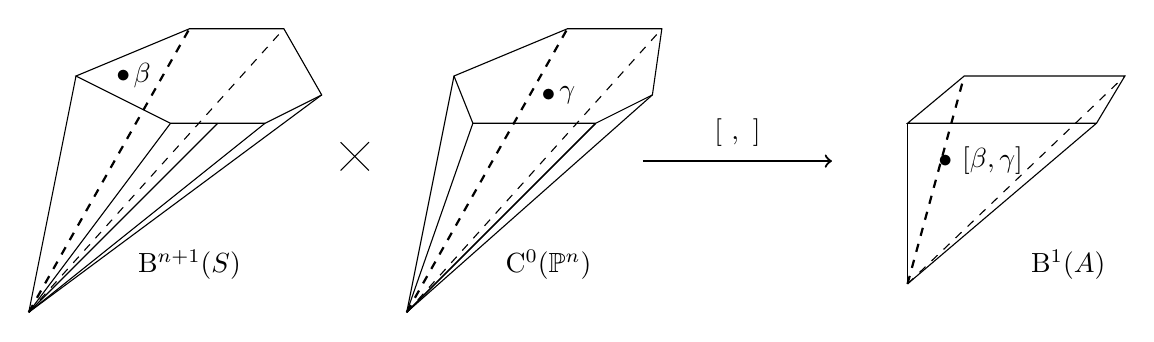
\begin{tikzpicture}[scale=1.2]
%% first cone
\draw[-](.5,.5)--(1,3);
\draw[-](.5,.5)--(2,2.5);
\draw[-](.5,.5)--(3,2.5);
\draw[-](.5,.5)--(3.6,2.8);
\draw[-](.5,.5)--(2.5,2.5);
\draw(1.5,3.0) node {$\bullet$};
\draw(1.7,3.0) node {$\beta$};
\draw(2.2,1.0) node {$\BBQ^{n+1}(S)$};
\draw[dashed,-](.5,.5)--(3.2,3.5);
\draw[dashed,-,thick](.5,.5)--(2.2,3.5);
\draw[-](1,3)--(2,2.5)--(3,2.5)--(3.6,2.8)--(3.2,3.5)--(2.2,3.5)--cycle;
%% the cross
\draw[-] (3.8,2)--(4.1,2.3);
\draw[-] (4.1,2)--(3.8,2.3);
%% second cone
\draw[-](4.5,.5)--(5,3);
\draw[-](4.5,.5)--(5.2,2.5);
\draw(6.0,2.8) node {$\bullet$};
\draw(6.2,2.8) node {$\gamma$};
\draw(6.0,1.0) node {$\CQ^0(\PP^{n})$};
\draw[-](4.5,.5)--(6.5,2.5);
\draw[-](4.5,.5)--(7.1,2.8);
\draw[-](4.5,.5)--(6.5,2.5);
\draw[dashed,-](4.5,.5)--(7.2,3.5);
\draw[dashed,-,thick](4.5,.5)--(6.2,3.5);
\draw[-](5,3)--(5.2,2.5)--(6.5,2.5)--(7.1,2.8)--(7.2,3.5)--(6.2,3.5)--cycle;
%%the arrow
\draw[->,thick](7,2.1)--(9,2.1);
\draw(8,2.4) node {$[\ , \ ]$};
%% third cone
%\draw[-](9.5,.5)--(10,3);
\draw[-](9.8,.8)--(9.8,2.5);
\draw[-](9.8,.8)--(11.8,2.5);
%\draw[-](9.5,.5)--(10.4,2.8);
%\draw[-](9.5,.5)--(11.5,2.5);
\draw[dashed,-](9.8,.8)--(12.1,3.0);
\draw[dashed,-,thick](9.8,.8)--(10.4,3.0);
\draw(10.2,2.1) node {$\bullet$};
\draw(10.7,2.1) node {$[\beta,\gamma]$};
\draw(11.5,1.0) node {$\BBQ^{1}(A)$};
\draw[-](9.8,2.5)--(11.8,2.5)--(12.1,3.0)--(10.4,3.0)--cycle;
\end{tikzpicture}
\caption{The ``duality'' between Betti tables and cohomology tables involves three cones.  Namely, given the Betti table $\beta(\FF)$ of a complex of free $S$-modules, and the cohomology table $\gamma(\cE)$ of a complex of coherent sheaves on $\PP^n$, our pairing produces the Betti table $\beta(\Phi(\FF,\cE))$ of a complex free $A$-modules.
}
\label{fig:bracket}
\end{figure}

The target of the above pairing, the cone of Betti tables on $A$ with finite length homology (which we denote $\BBQ^1(A)$), is easy to describe, and it is easy to write down the positive functionals that define it.
The functor $\Phi$ induces all the pairings defined by Eisenbud and Schreyer: by composing $\Phi$ with a nonnegative functional on $\BBQ^1(A)$, we get all the functionals $\langle -,-\rangle_{\tau,\kappa}$ used by Eisenbud and Schreyer.

As noted above, working with the derived category $\DD^b(S)$ instead of minimal free resolutions represents a shift in perspective for Boij--S\"oderberg theory.  This shift is essential, as the functor $\Phi$ does not respect the property of being a resolution: if $\FF$ is a resolution of a finite length module, then $\Phi(\FF,\cE)$ will be a complex of $A$-modules with finite length homology, but it will generally fail to be a resolution.  


\addtocontents{toc}{\protect\setcounter{tocdepth}{-1}}
\subsection*{Comparing Complexes and Resolutions}
\addtocontents{toc}{\protect\setcounter{tocdepth}{1}}
%\subsecNTOC{Comparing Complexes and Resolutions}
Here is a consequence of the analysis of Betti tables allowed by this categorification: If every bounded complex of free $S$-modules were quasi-isomorphic to its homology---which is not the case except when $n=0$, that is $S$ is the polynomial ring in just 1 variable---then the Betti table of a complex would be the sum of the Betti tables of the resolutions of its homology.  We show that, in great generality, the Betti table is  a sum of Betti tables of resolutions, but with rational, not integral coefficients, and not necessarily of the original homology modules. 

Here, for simplicity, is the special case of this result when the homology has finite length. 
%
%\begin{cor}\label{cor:decompose}
%Let $\FF\in \DD^b(S)$.  If $\FF$ 
%\begin{enumerate}
%	\item  If $\FF$ has finite length homology, then $\beta(\FF)$ may be written as a positive rational combination of Betti tables of shifted free resolutions
%	\[\beta(\FF)=\sum_{i=0}^s \beta(M^i)[i]\]
%	 where each module $M^i$ has finite length.
%	\item  If $\codim H^i\FF\geq i$ then $\beta(\FF)$ may be written as a positive rational combination of Betti tables of shifted free resolutions
%\[\beta(\FF)=\sum_{i=0}^s \beta(M^i)[i]\]
%where $\codim(M^i)\geq i$ for all $i$.
%\end{enumerate}
%As in the case of resolutions, the decomposition is algorithmic and, in a certain sense, unique.	
%\end{cor}
\begin{cor}\label{cor:decompose}
Let $\FF\in \DD^b(S)$ have finite length homology.  Then $\beta(\FF)$ is a positive rational combination of Betti tables of shifted free resolutions of modules of finite length (as in the case of resolutions, the decomposition is algorithmic and, in a certain sense, unique.)
\end{cor}

Similar statements hold for any $\FF\in \DD^b(S)$.  Theorem~\ref{thm:extremal rays refined} provides the full statement and proof, which implies the known results about decompositions of Betti tables
of minimal free resolutions from \cites{eis-schrey1,boij-sod2}.
The denominators of the coefficients involved in the decomposition may be seen as a measure of the extent to which the complex is not quasi-isomorphic to its homology. 

By convention we display the Betti table of $\FF$ as a table
of integers where the element of the $i$-th column and $j$-th row is $\beta_{i,i+j}\FF$, and we replace each zero with $-$. For clarity we often decorate the $(0,0)$ entry
with a superscript $\circ$.

\begin{example}
Let $S=\kk[x,y]$ and consider the complex:
\[
\FF := \left[S^1\overset{\left(\begin{smallmatrix}x&y\end{smallmatrix}\right)}{\xlongleftarrow{\hspace*{1.1cm}}} S^2(-1)\overset{\left(\begin{smallmatrix}-y^2&xy\\xy&-x^2\end{smallmatrix}\right)}{\xlongleftarrow{\hspace*{1.1cm}}} S^2(-3)\overset{\left(\begin{smallmatrix}y\\x\end{smallmatrix}\right)}{\xlongleftarrow{\hspace*{1.1cm}}} S^1(-4)\right],
\]
which has finite length homology $H_{0}\FF = \kk,\ H_{1}\FF = \kk(-2)$, and the minimal free resolution of $S/(x,y)^{2}$, which 
is
\[
\bG := 
\left[S^1\overset{\left(\begin{smallmatrix}x^{2}&xy&y^{2}\end{smallmatrix}\right)}
{\xlongleftarrow{\hspace*{1.1cm}}} 
S^3(-2)\overset{\left(\begin{smallmatrix}y&0\\-x&y\\0&-x\end{smallmatrix}\right)}{\xlongleftarrow{\hspace*{1.1cm}}} S^2(-3)\right].
\]
The Betti table
$$
\beta(\FF)=\begin{pmatrix} 1^\circ&2&-&-\\-&-&2&1\end{pmatrix}
$$
decomposes as a rational combination of the Betti table of $\bG$ shifted in 
homological degree by 1,
$$
\beta(\bG[1]) =\begin{pmatrix} -^{\circ}&1&-&-\\-&-&3&2\end{pmatrix},
$$
and the Betti table of the dual of $\bG$, 
$$
\beta(\bG^{*}) = \begin{pmatrix} 2^\circ&3&-\\-&-&1\end{pmatrix}.
$$
In fact, as one sees immediately,
\[
\beta(\FF)=
\frac{1}{2}\beta(\bG[1])
+
\frac{1}{2}\beta(\bG^{*}).
\]
By contrast, $\beta(\FF)$ \emph{cannot} be written as a positive \emph{integral} combination of Betti tables of resolutions of modules of finite length: by Hilbert's Syzygy Theorem the Betti table of $\FF$  is not equal to any Betti table of a resolution, since $\FF$ has length 3; and the sum of the Betti numbers of any resolution of a nonzero module of finite length is at least 4, while the sum of the Betti numbers of $\FF$ is $6<2\cdot 4$.
\end{example}



%%%%%%%%%%%%%%%%%%%%%%%%%%%%%%
\subsection*{Beyond Polynomial Rings}
%%%%%%%%%%%%%%%%%%%%%%%%%%%%%%
%%%%%%%%%%%%%%%%%%%%%%%%%%%%%%
Our description of the cone of Betti tables of bounded complexes
extends to a wide class of rings in the following way. Let $f:X\to \PP^{n}$ be a finite
morphism from a projective variety of dimension $n$, and set $L:=f^*\cO(1)$. 
Write $R=R(X,L)=\oplus_{e\in \mathbb N} H^0(X,L^{\otimes e})$ for the \defi{section ring}
of $L$.

We say that $\cU$ is an \defi{Ulrich sheaf} for $f$ if $f_*(\cU)\cong \cO_{\PP^n}^r$ for some $r>0$.  It was pointed out in \cite[Theorem~5]{eis-schrey-abel} that the existence of an Ulrich sheaf for $f$ implies that  the cone of cohomology tables of vector bundles on $X$ is the same as that on $\PP^{n}$. (The theorem is stated there in the special case when $L$ is very ample, but the proof
carries over to this more general situation.) The situation for Betti tables of resolutions over $R$ is not at all analogous to the situation of resolutions over $S$. But we prove a complete analogy for bounded complexes with finite length homology:

\begin{cor}\label{cor:isom cones}
If $f:X\to \P^{d}$ is a  finite map from an $d$-dimensional variety and $X$ admits an Ulrich sheaf for $f$, then the cone of Betti tables
of bounded free complexes with finite length homology over  the section ring
of $R(X,f^*\cO_{\PP^d}(1))$ is the same
as the cone of complexes with finite length homology on $S$. 
\end{cor}

\begin{example}\label{ex:elliptic}
Let $E$ be an elliptic curve and let $L=2P$, where $P$ is any point of $E$.  The map $f$ corresponding to the complete
linear series $|L|$ maps $E$ two-to-one to $\P^{1}$. The ring $R(E,L)$ has the form
$\kk[x_1,x_2,y]/(g(x_{1},x_{2},y))$  where $\deg(x_i)=1$, $\deg(y)=2$, and where $\deg(g)=4$.
If $P\neq Q\in E$ then the sheaf $L(P-Q)$ is an Ulrich sheaf for $f$. Thus the cone of
Betti tables of bounded free complexes with finite length homology over $R$ is the same
as the corresponding cone over $\P^{1}$.

The bundle $L$ in Corollary~\ref{cor:isom cones} must be ample, since the map $L$ is finite.  However, the theorem is not true for an arbitrary ample bundle.  For example, let $P$ be a point on an elliptic curve $E$, and let $R=R(E,P)$.  Since $\dim R_1=h^0(E,\cO_E(P))=1$, there cannot exist a pure complex:
\[
0\gets R^1\gets R^2(-1)\gets R(-2)\gets 0
\]
with finite length homology.
\end{example}

For many of the graded rings $R$ covered by Corollary~\ref{cor:isom cones}, there exist finitely generated $R$-modules of infinite projective dimension.  It would thus be natural to consider bounded below elements of the derived category of graded $R$-modules.  In \S\ref{sec:infinite}, we take a different approach: by realizing an infinite resolution as a limit of bounded complexes, we apply our results to prove a decomposition theorem for the Betti table of any such infinite resolution.

\subsection*{The Multigraded Case}
The functor $\Phi$ naturally generalizes to the multigraded case, offering the possibility of extending Boij--S\"oderberg theory to toric varieties.  Let $X$ be any projective toric variety with $\rank \Pic(X)=m$.  Let $R$ be the Cox Ring of $X$, presented as an $\mathbb N^m$-graded ring, and let $I$ be the irrelevant ideal of $R$.  Let $C=\kk[t_1, \dots, t_m]$ be $\mathbb N^m$-graded with irrelevant ideal $(t_1t_2\cdots t_m)$.  We say that a complex $\FF$ over $R$ or $C$ has \defi{irrelevant homology} if its homology is supported on the irrelevant ideal.

Let $\DD^b(R)$ and $\DD^b(C)$ denote the bounded derived categories of finitely generated, multigraded $R$-modules and $C$-modules, respectively.   For $\FF\in \DD^b(R)$ or in $\DD^b(C)$, $i\in \ZZ$, and $\alpha\in \ZZ^m$, we define the multigraded Betti numbers by the formula $\beta_{i,\alpha} \FF:=\dim \Tor_i(\FF,\kk)_{\alpha}$.  Similarly, for $\cE\in \DD^b(X), i\in \ZZ$ and $\alpha\in \ZZ^m$, we define multigraded cohomology numbers by the formula $\gamma_{i,\alpha} \cE:=\dim H^i(X, \cE(\alpha))$.  


For  $\FF\in \DD^b(R)$, let $\widetilde{\FF}$ denote the corresponding complex of coherent sheaves in $\DD^b(X)$.  There exists a functor
\[
\Phi': \DD^b(R)\times \DD^b(X)\to \DD^b(C)
\]
with the following properties:
\begin{theorem}\label{thm:Phimulti}
\begin{enumerate}
	\item\label{thm:Phi':1}  The multigraded Betti table of $\Phi'(\FF,\cE)$ depends only on the multigraded Betti table of $\FF$ and the multigraded cohomology table of $\cE$.
	\item\label{thm:Phi':2}  If $\widetilde{\FF}\otimes \cE$ is exact, then $\Phi'(\FF,\cE)$ has irrelevant homology.  This occurs, for instance, whenever $\FF$ is a complex with irrelevant homology and when $\cE$ is a vector bundle.
\end{enumerate}
\end{theorem}



The functor $\Phi'$ thus yields bilinear pairings relating multigraded Betti tables and multigraded cohomology tables, including a pairing of the form:
\begin{equation*}%\tag{**}
\label{eqn:multipairing}
%
\left\{\begin{matrix}
%\text{Cone generated by}\\
\text{Betti tables of} \\ \text{free $R$-complexes with}\\
\text{  irrelevant homology}\end{matrix}\right\}
%
\times 
%
\left\{\begin{matrix}
%\text{Cone generated by}\\
\text{cohomology }\\
\text{tables of vector}\\
\text{ bundles on } X
\end{matrix}\right\}
%
\longrightarrow
\left\{\begin{matrix}
%\text{Cone generated by}\\
\text{Betti tables of} \\ \text{free $C$-complexes with}\\
\text{  irrelevant homology}
\end{matrix}\right\}
\end{equation*}
It seems from this that the cone of free $R$-complexes with irrelevant homology will be easier to study than the cone of free $R$-complexes with finite length homology.  \daniel{For $C$, the statement is actually relatively clear.  For $R$ it is more speculative.  This is maybe best discussed over the phone.}

\subsection*{Structure of this paper}
\david{rewrite this when the paper settles down.} 
 The duality pairing is considered in detail in \S\ref{sec:duality pairing}. In \S\ref{sec:PP0} we analyze the cone $\BBQ^1(A)$ in detail, which provides a sort of base case for our positivity and duality statements.  We prove our main results in \S\ref{sec:general case}.  We then briefly discuss applications to the study of free resolutions in \S\ref{sec:refined}.  Finally, in \S\ref{sec:functor}, we extend these results to new polarized varieties and graded rings.

%%%%%%%%%%%%%%%%%%%%%%%%
%%%%%%%%%%%%%%%%%%%%%%%%
\addtocontents{toc}{\protect\setcounter{tocdepth}{-1}}
\section*{Acknowledgments}
\addtocontents{toc}{\protect\setcounter{tocdepth}{1}}
%%%%%%%%%%%%%%%%%%%%%%%%
%%%%%%%%%%%%%%%%%%%%%%%%
We thank Ezra Miller, Christine Berkesch, Ravi Vakil, Rob Lazarsfeld, Bhargav Bhatt,\dots



%%%%%%%%%%%%%%%%%%%%%%%%
%%%%%%%%%%%%%%%%%%%%%%%%
\section*{Part I: Categorifying the Duality in Boij-S\"oderberg Theory}
%%%%%%%%%%%%%%%%%%%%%%%%
%%%%%%%%%%%%%%%%%%%%%%%%
\section{Background and Notation}\label{sec:notation}
%%%%%%%%%%%%%%%%%%%%%%%%
%%%%%%%%%%%%%%%%%%%%%%%%
We gather some notation and definitions that we will use throughout.  We set $\mathfrak m=(x_0, \dots, x_n)$ to be the homogeneous maximal ideal on $S$.
\begin{defn}
If $\FF\in \DD^b(S)$ is a free complex, then we say that $\FF$ is \defi{minimal} if each differential $\partial: \FF_i\to \FF_{i-1}$ satisfies $\partial(\FF_i)\subseteq \mathfrak m\FF_{i-1}$.
\end{defn}
We may represent any $\FF\in \DD^b(S)$ by a minimal, free complex.  Under this assumption, we may write $\FF_i$ as the direct sum $\FF_i=\oplus_{j\in \ZZ} S(-j)^{\beta_{i,j}\FF}$.  If $\FF$ is quasi-isomorphic to a complex with only one nonzero term, then we say that $\FF$ is a \defi{shifted resolution}.


\begin{defn}
A \defi{shifted degree sequence of codimension $\ell$} is a sequence
\[{\bf d}=(\dots, d_i, d_{i+1}, \dots)
\]
with  $d_{i} \in \{\emptyset\}\cup \ZZ\cup \{\infty\}$ and $d_i \leq d_{i+1}-1$, where we make the convention that $\emptyset<d$ for any $d\in \ZZ$, and 
where there are precisely $\ell+1$ entries of $d$ lying in $\ZZ$. 
We define a partial order on shifted degree sequences by the termwise partial order, so $d\leq d'$ if $d_i\leq d_i'$ for all $i$.

As with Betti tables, we use a $\zp$ to indicate homological position zero when writing a degree sequence. 
\end{defn}



Thus for example
$$
(\dots, \emptyset , 0, 1^{\circ}, 3, \infty, \dots) < (\dots, \emptyset , 0, 1, 3^{\circ}, \infty, \dots) 
$$
are shifted degree sequences of codimension 2.

Given any degree sequence $d$, we say that a complex $\FF$ is \defi{pure of type $d$} if, for all $i$ such that $d_i\in \ZZ$, the free module $\FF_i$ is generated entirely in degree $d_i$.   The existence of pure resolutions (see~\cite{efw} or \cite[\S5]{eis-schrey1}) shows that, for any shifted degree sequence $d$ of codimension $\ell\leq n+1$, there exists a shifted resolution of a Cohen-Macaulay module over $S$ that is a pure complex of type $d$.  One of the central results of Boij--S\"oderberg theory is that the Betti tables of pure resolutions correspond bijectively with the extremal rays of cone of Betti tables of minimal free resolutions.  In other words, if $\FF$ is a minimal free resolution, then $\beta(\FF)$ may be written as a positive rational combination of the Betti tables of pure resolutions.  See~\cite{eis-schrey-icm,floystad-expository} for expository introductions to Boij--S\"oderberg theory.  We remark that, in \S\ref{sec:refined}, we introduce new notation for discussing many different cones of Betti tables.


If $P$ is some property that may be applied to a graded $S$-module, we extend the definition to the derived category by saying that $\FF \in \DD^b(S)$ has property $P$ if the direct sum of the homology modules of $\FF$ have this property. We similarly take the definition of any property that may be applied to a coherent sheaf, and we extend this to any $\cE\in \DD^b(\PP^n)$.  

A \defi{root sequence of dimension $\ell$} is a sequence $f=(f_1,\dots,f_\ell)\in \mathbb Z^{\ell}$ with $f_i\geq f_{i-1}+1$ for all $i$.  
A sheaf $\cE$ on $\PP^{n}$ is
\defi{supernatural of type} $f=(f_1, \dots, f_{s})$ if the following are satisfied: 
\begin{enumerate}
\item The dimension of $\cE$ is $s$.
\item For all $j\in \mathbb Z$, there exists at most one $i$ 
		such that $\dim_\Bbbk H^i(\PP^{n}, \cE(j))\ne 0$.
\item The Hilbert polynomial of $\cE$ has roots $f_1, \dots, f_{s}$.
\end{enumerate}
For every root sequence $f$, there exists a supernatural sheaf of type
$f$~\cite[Theorem~0.4]{eis-schrey1}.
Moreover, the cohomology table of any coherent sheaf 
can be written as a positive real combination of cohomology tables 
of supernatural sheaves~\cite[Theorem~0.1]{eis-schrey1}.  

One of the main results of \cite{eis-schrey1} indicates a duality between the cone of Betti tables of free resolutions of finite length graded $S$-modules and the cone of cohomology tables of vector bundles on $\PP^n$.  We provide a new perspective on this duality in \S\ref{sec:duality}. 


\begin{defn}
We index complexes in $\DD^b(S)$ homologically as in $\FF=[\dots \gets \FF_0\gets \FF_1\gets \dots]$.  For any $k\in \ZZ$, we define a \defi{shift} of $\FF$, denoted $\FF[k]$, as the complex obtained by shifting the indices in the following way:  $(\FF[k])_i=\FF_{i-k}$.
\end{defn}


%%%%%%%%%%%%%%%%%%%%%%%%
%%%%%%%%%%%%%%%%%%%%%%%%
\section{The Pairing $\Phi$}\label{sec:duality pairing}
%%%%%%%%%%%%%%%%%%%%%%%%
%%%%%%%%%%%%%%%%%%%%%%%%
In this we define the functor $\Phi$ and we prove Theorem~\ref{thm:Phi} describing its main properties.  As before, set $A= \kk[t]$. Let 
$\sigma: S\to S\otimes A = S[t]$
be the homomorphism defined by $\sigma(x_{i})=x_{i}t$. 
We write $-\otimes_\sigma S[t]$ to denote tensoring over $S$ with $S[t]$ using the structure
given by $\sigma$. Note that $\sigma$ is not a flat map---it is not even equidimensional.

If $F$ is a graded  $S$-module, then 
$$
F\otimes_{\sigma} S[t]
$$
is a bigraded $S[t]$ module.
Thus we may define a functor $\tau$ on derived
categories that takes a graded complex of free $S$-modules $\FF$ to
$$
\tau(\FF): =\widetilde \FF \otimes_{\sigma}\cO_{\PP^{n}\times \AA^{1}},
$$
a complex of graded sheaves on $\PP^{n}\times \AA^{1}$, with the grading coming from degree in $t$, the coordinate on $\AA^{1}$. For example, if 
$$
\FF: 0\rTo S(-d)\rTo^{f}S\rTo 0
$$
where $f$ is a form of degree $d$, then
$$
\tau(\FF): 0\rTo \cO_{\PP^{n}}(-d)\boxtimes A(-d)\rTo^{t^{d}f}\cO_{\PP^{n}}\boxtimes A \rTo 0
$$
where $P\boxtimes Q$ denotes the tensor product of the pullbacks of $P$ and $Q$ from
$\PP^{n}$ and $\AA^{1}$, respectively. This description of $\tau$ could 
be extended to graded complexes of arbitrary finitely generated graded modules
at the expense of replacing the tensor product with a derived tensor product, but we
will never need this.

%\begin{defn} The functor $\Phi: D^{b}(\P^{n}) \times D^{b}(S) \to D^{b}(A)$ is given by:
%$$
%\Phi(\cE,\FF) = R\pi_{*} \left(\tau_{0}(\cE)\otimes_{\P^{n}\times\AA^{1}} \tau_{1}(\FF)\right)
%$$
%where $\pi: \PP^{n}\times \AA^{1}\to \AA^{1}$ is the projection.
%\end{defn}

\begin{defn} \label{defn:product} The functor $\Phi: \DD^{b}(S)\times \DD^b(\PP^n) \to \DD^{b}(A)$ is given by:
$$
\Phi(\FF,\cE) = Rp_{2*} \bigl(\tau(\FF)\otimes_{\P^{n}\times\AA^{1}} (\cE\boxtimes \cO_{\AA^{1}}) \bigr)
$$
where $\FF$ denotes a graded  complex of finitely generated free $S$-modules and
$p_2: \PP^{n}\times \AA^{1}\to \AA^{1}$ is the projection. We will often write
$\FF\cdot \cE$ for $\Phi(\FF,\cE)$.
\end{defn}
We sometimes omit $\Phi$ from the notation, and simply write 
$\FF\cdot \cE:=\Phi(\FF,\cE)$.

For those comfortable with stacks, Definition~\ref{defn:product}
could be rephrased as follows. Consider the commutative diagram:
\[
\xymatrix{
\PP^n&\PP^{n}\times [\AA^1/\GG_m]\ar[l]_-{\pi_{1}} \ar[r]^-{\Sigma} \ar[d]^{\pi_2}&[\AA^{n+1}/\GG_m]\\
&[\AA^1/\GG_m]&%[\Spec(\kk)/\GG_m]\ar[l]_{o}
}
\]
where $\Sigma$ is the morphism induced by $\sigma$ and the maps $\pi_1$ and $\pi_2$ are the projections.  We could define $\Phi(\FF,\cE)$ to be $R\pi_{2*}\left( \Sigma^*\FF\otimes \pi_{1}^{*}\cE\right)\in \DD^b([\AA^1/\GG_m])$.

To see why this is an equivalent definition, note first  that there is an equivalence of categories (given by pullback/descent) between coherent sheaves on $[\AA^1/\GG_m]$ and graded, finitely generated $A$-modules. Further, since the covering map $\AA^1\to [\AA^1/\GG_m]$ is flat, cohomology commutes with base change (see \cite[0765]{stacks-project}) for the diagram
\[
\xymatrix{
\PP^n\times \AA^1\ar[r]\ar[d]^-{p_2}&\PP^{n}\times [\AA^1/\GG_m]\ar[d]^{\pi_2}\\
\AA^1\ar[r]&[\AA^1/\GG_m].
}
\]
Thus, the pullback of $R\pi_{2*}\left( \Sigma^*\FF\otimes \pi_{1}^{*}\cE\right)$ is quasi-isomorphic 
to $\Phi(\FF,\cE)$ as defined in Definition \ref{defn:product}.

Here is a sample computation of $\Phi$: 

\begin{example} Let 
$$
\bK = \bigl[ S\lTo S^{n+1}(-1) \lTo \wedge^{2}(S^{n+1})(-2) \lTo\cdots\lTo S(-n-1)\bigr]
$$
be the Koszul complex, the minimal free resolution of $\kk$, and take
$\cE = \cO_{\PP^{n}}$, so that 
$$
\bK \cdot \cE = Rp_{2*}\tau(\bK).$$  
There is a spectral sequence converging to $Rp_{2*}(\widetilde {\sigma^{*}\bK})\otimes \cE$
whose $^{2}E$ page has in the $(i,j)$ position the $i$-th homology of the complex
of $j$-th cohomology modules of the terms in $\bK$. But since
$$
\widetilde {\sigma^{*} S(-a)} \cong \cO_{\PP^{n}}(-a)\otimes A(-a),
$$
the terms on this page all vanish except for
$$
H^{0} (\widetilde{\bK_{0}}) = H^{0}(\cO_{\PP^{n}}\boxtimes A) = A,
$$
in cohomological degree 0, and 
$$
H^{n}(\widetilde{\bK_{n+1}}) = H^{n}(\cO_{\PP^{n}}(-n-1)\boxtimes A(-n-1) = A(-n-1)
$$
in cohomological degree $n-(n+1) = -1$.
Thus the complex $\bK \cdot \cE$ has the form
$$
A\lTo^{ut^{n}}A(-n)
$$
for some $u\in \kk$. But the complex $\FF$ has homology of finite length, so the complex $\sigma^{*}\FF \otimes p_{2}^{*}\cE$ has homology annihilated by a power of $t$, and thus $\FF\cdot \cE$ will also have homology annihilated by a power of $t$. It follows that $u\neq 0$, and $\FF\cdot \cO_{\PP^{n}}$ is quasi-isomorphic to the graded $A$-module $A/(t^{n})$, regarded as a complex concentrated in homological degree 0.
\end{example}


%%%%%%%%%%%%%%%%%%%%%%%%%
%%%%%%%%%%%%%%%%%%%%%%%%%
%\section{The Betti table of $\Phi(\FF,\cE)$}\label{sec:Betti of Phi}
%%%%%%%%%%%%%%%%%%%%%%%%%
%%%%%%%%%%%%%%%%%%%%%%%%%
\daniel{I combined the section defining $\Phi$ with the section decsribing the Betti table of $\Phi(\FF,\cE)$.  We can easily go back\dots}
The following result, which is a strengthened version of Theorem~\ref{thm:Phi}\eqref{thm:Phi:1}.
\begin{theorem}\label{thm:betti numbers of pairing}
The Betti numbers of $\FF\cdot \cE = \Phi(\FF,\cE)$ are given by the formula:
\[
\beta_{i,j}(\FF\cdot \cE)=\sum_{p-q=i}  \beta_{p,j}(\FF)\gamma_{q,-j}(\cE).
\]
In particular, the Betti table of $\FF\cdot \cE$ only depends on $\beta(\FF)$ and $\gamma(\cE)$.
\end{theorem}


\begin{proof}
Without loss of generality, we assume that $\FF$ is supported entirely in nonnegative homological degrees, so that $\FF=[\FF_0\gets \dots \gets \FF_p]$.  
We may compute $\FF\cdot \cE$ explicitly in terms of a certain spectral sequence for computing $Rp_{2*}$.  First, we consider the double complex $C_{\bullet, \bullet}$ where $C_{i,\bullet}$ is the Cech resolution of $\widetilde{\FF'}_i\otimes \cE'$ on $\PP^n_A$ with respect to the standard Cech cover of $\mathbb P^n$.  If we represent all of the maps in $C_{\bullet, \bullet}$ with matrices, then all of the vertical maps (which are induced by the Cech resolutions) will involve degree $0$ elements, and all of the horizontal maps (which are induced by the maps in $\rho^*\FF$) will involve bihomogeneous elements that are strictly positive in both bidegrees.

Since $\Tot(C_{\bullet, \bullet})$ is a complex of flat $A$-modules that is quasi-isomorphic to $\FF\cdot \cE$, we can obtain the Betti numbers by computing $\Tor(\Tot(C_{\bullet, \bullet}), A/(t))$.  When we tensor by $A/(t)$, the vertical maps of $C_{\bullet, \bullet}$ are unchanged, but the horizontal maps all go to $0$.  
Hence, one spectral sequence degenerates, so the $i$th homology of $\Tot(C_{\bullet,\bullet})/(t)$ equals the sum 
\[
\HH^i(\Tot(C_{\bullet,\bullet})/(t))\cong \bigoplus_{j} \HH^j_{\text{vert}}(C_{i+j,\bullet})
\]

Now we compute the other spectral sequence.
Recall that $\FF_i=\oplus_{j\in \ZZ} S(-j)^{\beta_{i,j}(\FF)}$.  For brevity, we use $\beta_{i,j}:=\beta_{i,j}(\FF)$, and we may write $\FF_i'\otimes \cE\cong \bigoplus_{j\in \ZZ} \cE(-j)^{\beta_{i,j}}\boxtimes A(-j)^{\beta_{i,j}}$.

After taking the vertical homology of $C_{\bullet, \bullet}$, we obtain:
\[
\xymatrix{
\bigoplus_{j} H^n(\cE(-j)^{\beta_{0,j}})\otimes A(-j)^{\beta_{0,j}}&\bigoplus_{j} H^n(\cE(-j)^{\beta_{1,j}})\otimes A(-j)^{\beta_{1,j}}\ar[l]&\dots\ar[l]\\
\vdots & \vdots&\\
\bigoplus_{j} H^1(\cE(-j)^{\beta_{0,j}})\otimes A(-j)^{\beta_{0,j}}&\bigoplus_{j} H^1(\cE(-j)^{\beta_{1,j}})\otimes A(-j)^{\beta_{1,j}}\ar[l]&\dots\ar[l]\\
\bigoplus_{j} H^0( \cE(-j)^{\beta_{0,j}})\otimes A(-j)^{\beta_{0,j}}&\bigoplus_{j} H^0(\cE(-j)^{\beta_{1,j}})\otimes A(-j)^{\beta_{1,j}}\ar[l]&\dots\ar[l]
}
\]
We conclude that
\[
\Tor^i_A(\FF\cdot \cE, A/(t))\cong \HH^i(\Tot(C_{\bullet,\bullet})/(t))\cong \bigoplus_{p-q=i} \bigoplus_{j} H^q(\cO(-j)^{\beta_{p,j}}\otimes \cE)\otimes A(-j)^{\beta_{p,j}},
\]
which proves the formula.
\end{proof}


\begin{remark}\label{rmk:generic}
The proof of Theorem~\ref{thm:betti numbers of pairing} illustrates the following useful fact:  over the generic point of $\AA^1$, we have the isomorphism
\[
(\FF\cdot \cE)\otimes_{A} \kk(t)\cong \left( Rp_{2*}(\widetilde{\FF}\otimes \cE)\right) \otimes_{\kk} \kk(t).
\]
\end{remark}

As a Corollary of Theorem~\ref{thm:betti numbers of pairing}, we can recover the Betti numbers of a complex $\FF$  or the cohomology
table of a sheaf $\cE$ from the values of the pairing:
\begin{cor} 
We have:
\begin{enumerate}
\item 
 $\beta_{i,j}(\FF) = \beta_{i,j}(\FF\cdot \cO_{\P^{n}}(j))$ for all $i,j$, where $\cO_{\PP^n}(j)$ is regarded as a complex concentrated in homological degree 0.
\item $h^{i}(\cE(j)) = \beta_{-i,-j}(S(j)\cdot \cE)$, for all $i,j$, where $S(j)$ is regarded as a complex concentrated in homological degree 0.
\end{enumerate}
%\qed
\end{cor}


We will focus in this paper on free complexes, and we will need to use the definition of $\Phi$
only in the special case where $\cE$ is a vector bundle, or more generally a sheaf that is supported on some linear subspace of $\PP^{\ell}\subseteq \PP^n$ and that is a vector bundle when restricted to its support.

\begin{prop}\label{prop:exact}
Let $\FF\in \DD^b(S)$ and $\cE\in \DD^b(\PP^n)$.  If $\widetilde \FF\otimes \cE$ is exact, then the homology of the complex $\Phi(\FF,\cE)$ has finite length.
\end{prop}

\begin{proof} It suffices to show that the homology of $\Phi(\FF,\cE)$ is annihilated by
a power of $t$. After inverting $t$ the map $\sigma$ becomes the usual inclusion $S\subset S[t,t^{-1}]$
composed with the invertible change of variables $x_{i}\mapsto x_{i}t$. Thus the complex 
$$
\Gbull:=\bigl(\widetilde\FF\otimes_{\sigma}\cO_{\PP^{n}\times \Spec A[t,t^{-1}]}\bigr)
\otimes_{\PP^{n}\times \Spec A[t,t^{-1}]}
\cE \cong \widetilde \FF \otimes \cE \otimes \cO_{\Spec A[t,t^{-1}]}
$$
has no homology. It follows by a spectral sequence computation that 
the complex $R\pi_{2*}\GG$ on $\Spec A[t,t^{-1}]$ has no homology. By flat base change,
this is equal to the restriction of $\Phi(\FF,\cE)$ on the open set $t^{-1}$, and we see that the homology
of $\Phi(\FF,\cE)$ is annihilated by a power of $t$, as required.
\end{proof}

%%%%%%%%%%%%%%%%%%%%%%%%%%%%%%%%%%%%%%%%%
%%%%%%%%%%%%%%%%%%%%%%%%%%%%%%%%%%%%%%%%%
\section{Categorified Eisenbud--Schreyer Functionals}\label{sec:functionals}
%%%%%%%%%%%%%%%%%%%%%%%%%%%%%%%%%%%%%%%%%
%%%%%%%%%%%%%%%%%%%%%%%%%%%%%%%%%%%%%%%%%
We now illustrate how the pairing $\Phi$ provides a unifying view on all of the Eisenbud--Schreyer functionals and on the corresponding positivity results, including~\cite[Positivity 1]{eis-schrey-icm} and~ \cite[Positivity 2]{eis-schrey-icm}.  The basic idea breaks can be envisioned via Figure~\ref{fig:bracket}.  First, we use $\Phi$ and a supernatural bundle $\cE_f$ to obtain a map $\Phi(-,\cE_f)$ from Betti tables on $S$ to Betti tables on $A$.  Second, we analyze the functionals on $\DD^b(A)$ which are nonnegative when evaluated on complexes with finite length homology.  
This recipe provides lots of functionals that are nonnegative on Betti tables, including all of the Eisenbud--Schreyer functionals.

\begin{defn}\label{defn:chi}
Given $\Gbull\in \DD^b(A)$, we define $\chi_{i,j}(\Gbull)=\chi_{i,j}(\beta(\Gbull))$ as the dot product of the Betti table $\beta(\Gbull)$ with
\[
\chi_{i,j}:=
\left(
\begin{array}{cccccccc}
 & \vdots& &\multicolumn{1}{|c}{\vdots}&& \vdots&&\\
\dots&0&0&\multicolumn{1}{|c}{1}&-1&1&-1&\dots\\
\dots&0&0&\multicolumn{1}{|c}{1}&-1&1&-1&\dots\\
\dots&0&0&\multicolumn{1}{|c}{\mathbf{1}}&-1&1&-1&\dots\\ \cline{4-5}
\dots&0&0&0&0&\multicolumn{1}{|c}{1}&-1&\dots\\
\dots&0&0&0&0&\multicolumn{1}{|c}{1}&-1&\dots\\
& \vdots&&\vdots&& \multicolumn{1}{|c}{\vdots}&&\\
\end{array}
\right)
\]
where the boldface $1$ corresponds $\beta_{i,j}$, i.e. the boldface $1$ is in column $i$ and row $i-j$. 
\end{defn}
The line that snakes through
the table indicates how $\chi_{i,j}$ separates a Betti into two regions.  In the upper region, this is simply computing an Euler characteristic, and in the lower region, it is dot product with the zero matrix.

\begin{thm}\label{thm:categorified}
We have the following:
\begin{enumerate}
	\item  Let $\FF\in \DD^b(S)$ and $\cE\in \DD^b(\PP^n)$ with $\codim(\FF)+\codim(\cE)\geq n+1$.  Then
\[
\chi_{i,j}(\FF\cdot \cE)\geq 0
\]
	\item  Let $\cE_{f}$ be a supernatural sheaf of type $f=(f_1>\dots>f_s)$ on $\PP^n$.  Fix $1\leq \tau \leq s$ and let $\kappa=f_{\tau+1}-3$.  Let $\langle -, \cE_{f}\rangle_{\tau,\kappa}$ be the functional defined in \cite{eis-schrey-icm}, but extended in the natural way to a functional $\VV\to \QQ$ on the entire vector space $\VV$.  We then have an equality of functions
\[
\bigg( \beta(\FF)\mapsto \chi_{0,\kappa}(\FF\cdot \cE_f)\bigg) =\bigg( \beta(\FF)\mapsto \langle \FF, \cE_f\rangle_{\tau,\kappa} \bigg)\]
from $\VV \to \QQ$.
\end{enumerate}
\end{thm}
The above theorem illustrates the sense in which $\Phi$ categorifies all of the Eisenbud--Schreyer nonnegativity results, and it provides a unified perspective on the nonnegativity of all such functionals.  


\daniel{There's a lot of notation introduced below that we don't really use\dots This could be streamlined a lot probably.}
Our proof of the theorem relies on the relative simplicity of the derived category $\DD^b(A)$.  Because the global dimension of $A$ is 1, any element $\Gbull\in \DD^b(A)$ is quasi-isomorphic to its homology, and the homology $\HH(\Gbull)$ decomposes as
\begin{equation}\label{eqn:splitting}
\HH(\Gbull)=\left( \bigoplus_{i,j\in \ZZ} A(-j)[i]^{\lambda_{i,j}(\Gbull)}\right) \bigoplus \left( \bigoplus_{\substack{i,j\in \ZZ\\ k\in \ZZ_{>0}}} (A(-j)[i]/t^k)^{\nu_{i,j,k}(\Gbull)}\right),
\end{equation}
for uniquely defined nonnegative integers $\lambda_{i,j}(\Gbull), \nu_{i,j,k}(\Gbull)$.  Hence, as a monoid with respect to direct sum, $\DD^b(A)$ is isomorphic to a free abelian monoid on the countable set of generators $\{\lambda_{i,j} | i,j\in \ZZ\} \cup \{ \nu_{i,j,k}  | i,j\in \ZZ, k\in \ZZ_{>0}\}$. 

Note that a complex $\Gbull$ has finite length homology if and only if $\lambda_{i,j}(\Gbull)=0$ for all $i,j$.  We  define $\DD^b(A)_{\text{tor}}$ as the subcategory of complexes $\Gbull$ where $\lambda_{i,j}(\Gbull)=0$.  We use $\DD^b(A)\otimes_{\ZZ} \QQ$ and $\DD^b(A)_{\text{tor}}\otimes_{\ZZ} \QQ$ for the associated vector spaces.


The following lemma proves the nonnegativity of the functionals $\chi_{i,j}$ when restricted to $\DD^b(A)_{\text{tor}}\otimes_{\ZZ} \QQ$.  In \S\ref{sec:A} we provide a  complete analysis of the nonnegative functionals for cones of Betti tables over $A$.

\begin{lemma}\label{lem:chi nonneg}
If $\Gbull\in \DD^b(A)_{\text{tor}}$, then $\chi_{i,j}(\Gbull)\geq 0$.
\end{lemma}
\begin{proof}
\daniel{Can we add a one-sentence proof here along the lines of ``more generators than syzygies in any degree''?  This would be useful for quoting later in the toric/multigraded case.  I attempted such an argument (commented on in the TeX), but my argument dragged on and on.}
%Since $\Gbull$ has finite length homology, we may representative $\Gbull$ as direct sum of $2$-term shifted minimal free resolutions of finite length $A$-modules.  Thus, each minimal generator of $\Gbull$ may be uniquely partnered with another minimal generator.  A pair of generators $(m,m')$ contributes to this functional if $m'$ is a minimal generator of $\Gbull_{i+1}$ of degree $>j+1$ and if $m$ is either a minimal generator of $\Gbull_{i}$ of degree $\leq j$ or if $m$ is a minimal generator of $\Gbull_{i+2}$ of any degree.
%

More precisely, we claim that
\[
\chi_{i,j}(\Gbull)=\sum_{\substack{u,v,w \\ v< j+1<v+w}} \nu_{u,v,w}(\Gbull) + \sum_{\substack{u,v,w\\ t> j+1}} \nu_{u+1,v,w}(\Gbull).
\]
To check this claim, it suffices to evaluate both sides of the equation on $1$-term complexes $A(-v)[u]/t^w$, for all $u,v\in \ZZ$ and $w\in \ZZ_{>0}$, and the statement then follows.
\end{proof}

\begin{proof}[Proof of Theorem~\ref{thm:categorified}]
For part (1), we note that $\chi_{i,j}(\FF\cdot \cE)$ only depends on the Betti table of $\FF\cdot \cE$, which by Theorem~\ref{thm:Phi}\eqref{thm:Phi:1} only depends on $\beta(\FF)$ and $\gamma(\cE)$.  We may thus assume that $\kk$ is an infinite field and may replace $\cE$ by a general $\GL_{n+1}$ translate, since this does not affect the cohomology table of $\cE$.  By~\cite[Theorem]{miller-speyer}, we conclude conclude $\widetilde{\FF}\otimes \cE$ is exact.  Hence, by Theorem~\ref{thm:Phi}\eqref{thm:Phi:2}, it follows that $\FF\cdot \cE$ lies in $\DD^b(A)_{\text{tor}}$.  Finally, we apply Lemma~\ref{lem:chi nonneg} to obtain the desired nonnegativity.


The proof of part (2) follows from the argument of case (iii) of the proof of Theorem~\ref{thm:extremal rays refined}, given below.  
\end{proof}




\section*{Part II: Comparing Complexes and Resolutions}
%%%%%%%%%%%%%%%%%%%%%%%%%%%%%%%%%%%%
%%%%%%%%%%%%%%%%%%%%%%%%%%%%%%%%%%%%
\section{Complexes with Homology}\label{sec:refined}
%%%%%%%%%%%%%%%%%%%%%%%%%%%%%%%%%%%%
%%%%%%%%%%%%%%%%%%%%%%%%%%%%%%%%%%%%
The main result of this section and the next two is Theorem~\ref{thm:extremal rays refined}, which provides refined analogues of the main decomposition results in Boij--S\"oderberg, including those of \cites{eis-schrey1,boij-sod2} (see Example~\ref{ex:resolutions} below).  

\david{maybe we should allow unimodal sequences, to get at the monad case?}
\begin{defn} A \defi{codimension sequence} is a
a doubly infinite, nondecreasing or nonincreasing sequence 
$$
\bb=(\dots, b_{-1}, b_{0}^{\circ}, b_{1}, \dots )
$$
where  
$$
b_{i}\in \{\emptyset\} \cup \{0,1,\dots,n+1\}\cup \{\infty\}
$$
for each $i$, and we adopt the convention that $\emptyset<0$.   We say that a
minimal graded free complex $\FF$ over $S$ (or the element of $D^{b}(S)$ that it represents) is \defi{compatible with $\bb$} if 
\[
\codim \HH^i(\FF) \geq b_i, \text{ for all } i
\]
and if $\FF_i=0$ whenever $b_i=\emptyset$.
\end{defn}

\begin{example}
Let $\FF=[\FF_0\gets \dots \gets \FF_p]$ be the minimal free resolution of a module of codimension $c$.  The complex $\FF$ is compatible with $\bb=(\dots, 0,c-1^\circ,c,c+5,\dots)$.  However, $\FF$ is not compatible with $\bb=(\dots,c+1^\circ,c+1,\dots)$.  
\end{example}

Here are the cones of Betti tables and cohomology tables we will work with:
\begin{defn}\label{defn:cones}
We write $\BBQ^{\bb}(S)$ for the subcone of $\VV$ spanned by $\beta(\FF)$ as $\FF$ ranges over all elements of $\DD^b(S)$ that are compatible with $\bb$.  In case  $\bb_i=k$ for all $i$ we write $\BBQ^k(S)$ in place of $B^{\bb}(S)$.

For any $k=0, \dots, n$, we define $\CQ^k(\PP^n)$ to be the subcone of $\WW$ spanned by all $\cE\in \DD^b(\PP^n)$ satisfying $\codim(\cE)\geq k$.
\end{defn}

\begin{defn}\label{defn:deg compatible}
Suppose that $\bb$ is a nondecreasing (respectively nonincreasing) codimension sequence 
and ${\bf d}$ is a degree sequence  of codimension $\ell$. Let $k$ be the smallest index
such that $d_{k}\in \ZZ$. We say that $\dd$ is \defi{compatible with $\bb$} if $\bb_k\leq \ell\leq \bb_{k+1}$  (respectively, if $\bb_k\geq \ell\geq \bb_{k+1}$).
\end{defn}

Our main result is a description of the structure of a simplicial fan for $\BBQ^{\bb}(S)$ in terms of  Betti tables of pure resolutions.  

\begin{thm}\label{thm:extremal rays refined}
For any $\bb$ as above the cone $\BBQ^{\bb}(S)$ is locally polyhedral, and there is a natural bijection:
\[
\left\{
\begin{matrix}
\text{Extremal rays of }\\
\text{the cone } \BBQ^{\bb}(S)
\end{matrix}
\right\}
\longleftrightarrow
\left\{
\begin{matrix}
\text{Shifted degree sequences }\\
\text{ compatible with $\bb$}
\end{matrix}
\right\},
\]
where the shifted degree sequence $d$ corresponds to the ray spanned by 
the Betti table of any shifted pure free resolution of type $d$ of a Cohen-Macaulay module. Further, the cone $\BBQ^{\bb}(S)$ has a simplicial fan structure, where the simplices correspond to chains of shifted degree sequences.
\end{thm}

Here by the statement that $\BBQ^{\bb}(S)$ is \defi{locally polyhedral} we mean that if we fix any finite dimensional subspace $\VV_{\text{fin}}\subseteq \VV$ defined by the vanishing of coordinate vectors, then the restricted cone $\VV_{\text{fin}}\cap \BBQ^{\bb}(S)$ is polyhedral.  \daniel{There might be a cleaner way to say this, but the old definition was off b/c we still had infinite room for homological shifts.}

The proof of Theorem~\ref{thm:extremal rays refined} involves two essential steps.  First, in \S\ref{sec:A}, we provide a detailed description of cones of Betti tables on $A$.  Since $\DD^b(A)$ is the target of the pairing $\Phi$, these results will provide a base case for our main results.  Second, in \S\ref{sec:refined}, 
we use the nonnegative functionals obtained by combining  \S\ref{sec:A} with Theorem~\ref{thm:Phi} to complete the proof of Theorem~\ref{thm:extremal rays refined}. We postpone the details to the next section.

\begin{example}  
%There is a necessary subtlety in Definition~\ref{defn:deg compatible}, which is
%\emph{not} equivalent to asking that $\FF_d$ be compatible with $\bb$. 
%For instance, let

 Consider the codimension sequence $\bb=(\dots, \emptyset,0^\circ,0,\infty,\dots)$ and the degree sequence $\dd=(\dots, \emptyset,0^\circ ,1,\infty,\dots)$, which has codimension $\ell = 1$.  The Betti table 
 $(1^\circ, 1)$ of the complex $\FF=\left[ S^{1^\circ}\lTo^{x_{0}} S^1(-1)\right]$ is in $\BBQ^{\bb}$.
 As such, the decomposition guaranteed by Theorem~\ref{thm:extremal rays refined} is
 $\beta(\FF) = (1^{\circ}, -) + (-^{\circ}, 1)$. Of course we might also decompose $\beta(\FF)$
 as the Betti table $(1^{\circ}, 1)$ of a single pure resolution ($\FF$ itself!). This does \emph{not} contradict the uniqueness statement of the Theorem because $\dd$ is not compatible with $\bb$
 since $1= \ell \not\leq b_{1}= 0$.
\end{example}

%compatible with $\bb$
% 
% 
% , whereas the degree sequence $d$ is not compatible with $\bb$.
%
%This distinction is necessary in order to obtain the uniquesness of decompositions of Betti tables in Theorem~\ref{thm:extremal rays refined}.  Otherwise, in this case, $\FF_d$ would have two decompositions into pure tables:
%\[
%\beta(\FF_d)=\begin{pmatrix}
%1^\circ & 1
%\end{pmatrix}
%\quad \text{ or } \quad
%\beta(\FF_d)=
%\begin{pmatrix}
%1^\circ & -
%\end{pmatrix}
%+
%\begin{pmatrix}
%-^\circ & 1
%\end{pmatrix}.
%\]
%

\begin{cor}\label{cor:decompose refined}
Let $\bb$ be a nondecreasing or nonincreasing sequence, and let $\FF\in \DD^b(S)$ be compatible with $\bb$.  Then there exist modules $M^k$ of codimension $\geq \bb_k$ and nonnegative rational numbers $a_k\in \QQ_{\geq 0}$ such that
\[
\beta(\FF)=\sum_{k\in \ZZ} a_k\beta(M^k[k]).
\]
\end{cor}
As noted in the introduction, the denominators of the $a_k$ may be seen as a measurement of the extent to which $\FF$ fails to be quasi-isomorphic to its homology.  Several special cases of Theorem~\ref{thm:extremal rays refined} are of particular interest.

\begin{cor}\label{cor:uniform}
For any $k=0,\dots, n+1$, there is a natural bijection:
\[
\left\{
\begin{matrix}
\text{Extremal rays of }\\
\text{the cone } \BBQ^{k}(S)
\end{matrix}
\right\}
\longleftrightarrow
\left\{
\begin{matrix}
\text{Shifted degree sequences }\\
\text{ of codimension $k$}
\end{matrix}
\right\},
\]
where the shifted degree sequence $d$ corresponds to the ray spanned by the shifted pure resolution of type $d$ of a Cohen--Macaulay module. 
\end{cor}
In \S\ref{sec:duality} we use the functor $\Phi$ and the cones $\BBQ^k(S)$ to clarify the duality results of \cite{eis-schrey1}.


\begin{example}[Resolutions]\label{ex:resolutions}
%Let $\bb$ be the nondecreasing sequence $\bb=(\dots, \emptyset, n+1^*, \infty, \dots )$, where the asterisk indicates homological position $0$.  A complex $\FF$ is compatible with $\bb$ if and only if $\FF$ is the minimal free resolution of a finite length $S$-module.  Hence, for this value of $\bb$, Theorem~\ref{thm:extremal rays refined} recovers \cite[Theorem~0.2]{eis-schrey1}.
%
If $\bb=(\dots, \emptyset, 0^\zp, \infty, \dots)$ then a complex $\FF$ is compatible with $\bb$ if and only if $\FF$ is the minimal free resolution of an arbitrary $S$-module.  Hence, for this value of $\bb$, Theorem~\ref{thm:extremal rays refined} recovers the main results of \cite{boij-sod2}.
\end{example}
%
%
%\begin{example}[Complexes with finite length homology]\label{ex:fl hom}
%If $\bb=(\dots, n+1, n+1^\zp, n+1, \dots)$ then a complex $\FF$ is compatible with $\bb$ if and only if the homology modules of $\FF$ have finite length. Hence, for this value of $\bb$, Theorem~\ref{thm:extremal rays refined} implies Corollary~\ref{cor:decompose}.
%\end{example}

\begin{example}[Coresolutions]\label{ex:coresolutions}
Let $\bb$ be the nonincreasing sequence $\bb=(\dots, n+1, \dots, n+1, 0^\zp,\emptyset, \dots)$.  For any sheaf $\cE$ on $\PP^n$, let $\FF=[\FF_{-p}\gets \dots \gets \FF_0]$ be a positive, free complex such that 
\[
0\gets \widetilde{\FF}_{-p}\gets \dots \gets \widetilde{\FF}_0\gets \cE\gets 0
\]
is a coresolution of $\cE$.  Then $\FF$ is compatible with $\bb$ and hence $\beta(\FF)$ lies in $\BBQ^{\bb}(S)$.  

For instance, if $S=\kk[x_0, \dots, x_4]$ and $\cE=\bigwedge^3 \Omega_{\PP^4}$, then $\cE$ admits a coresolution:
\[
0\gets \cO_{\PP^4}\gets  \cO_{\PP^4}^5(-1)\gets  \cO_{\PP^4}^{10}(-2)\gets  \cO_{\PP^4}^{10}(-3)\gets \bigwedge^3 \Omega_{\PP^4}\gets 0.
\]
If $\FF$ is the corresponding positive, free complex of $S$-modules, then the decomposition of $\beta(\FF)$ into shifted pure diagrams compatible with $\bb$ is given by
\[
\beta(\FF)=\left(\begin{smallmatrix}-&-&-&-^\zp\\
-&-&-&-\\
-&-&-&-\\
1&5&10&10
\end{smallmatrix}\right)
=\left(\begin{smallmatrix}
-&-&-&-^\zp\\
-&-&-&-\\
-&-&-&-\\1&3&3&1
\end{smallmatrix}\right)
+
\left(\begin{smallmatrix}
-&-&-&-^\zp\\
-&-&-&-\\
-&-&-&-\\-&2&4&2^\zp
\end{smallmatrix}\right)
+
\left(\begin{smallmatrix}
-&-&-&-^\zp\\
-&-&-&-\\
-&-&-&-\\
-&-&3&3
\end{smallmatrix}\right)
+
\left(\begin{smallmatrix}
-&-&-&-^\zp\\
-&-&-&-\\
-&-&-&-\\
-&-&-&4
\end{smallmatrix}\right)
\]
Unlike the case of resolutions in Example~\ref{ex:resolutions}, there exist complexes $\FF$ compatible with $\bb$ such that $\widetilde{\FF}$ is not a coresolution of a coherent sheaf.  For instance, we could also realize $\beta(\FF)$ as above by taking direct sums of shifted Koszul complexes.
\end{example}

\begin{example}[Approximate resolutions]
Let $\bb=(\dots,\emptyset,0^\zp,n-1,n-1,\dots,)$.   Let $\FF\in \DD^b(S)$ be compatible with $\bb$ and let $M$ be the $0$th homology module of $\FF$.  We note that $\FF$ provides an approximate resolution of $M$, in the sense that the homology of $[\FF\to M]$ has dimension at most $1$.  Such approximate resolutions play a key role in \cite[Lemma~1.6]{gruson-lazarsfeld-peskine}, where they are used to bound the Castelnuovo--Mumford regularity of $M$.
\end{example}

\begin{example}[Monads]\daniel{This is a placeholder for the moment.  The first and second paragraphs don't match.  Namely, the first paragraph doesn't jive with the decomposition in the second paragraph.  But I think it may be fixable if we rewrite the first paragraph more carefully (splitting $\FF_0$ into two pieces).}
Given a sheaf $\cF$ on $\PP^n$, we recall that $\FF$ is a monad for $\cF$ if $\HH_0(\widetilde{\FF})\cong \cF$ and if $\HH_i(\widetilde{\FF})=0$ otherwise.  Note that $\FF_{\leq -1}$ is a coresolution (of $\ker\left(\widetilde{\FF}_{-1}\to \widetilde{\FF}_{-2}\right)$) and $\FF_{\geq 0}$ is a resolution (of $\coker\left(\widetilde{\FF}_{1}\to \widetilde{\FF}_{0}\right)$).  We may thus apply Examples~\ref{ex:resolutions} and \ref{ex:coresolutions} to provide a decomposition result for any such monad.

For instance, in \cite[Example 8.2]{eis-floy-schrey}, it shown that
\[
\widetilde{\FF}:=\left[0\gets \cO_{\PP^4}(-1)^2 \gets  \cO_{\PP^4}(-2)^{11}\gets \overset{\zp}{\cO_{\PP^4}(-3)^{20}}\gets \cO_{\PP^4}(-4)^{10}\gets 0 \right]
\]
is a monad for the ideal sheaf of a certain rational surface in $\PP^4$.  This decomposes as
\begin{align*}
\beta(\FF)&=
\begin{pmatrix}
2&11&20^\zp&10
\end{pmatrix}
\\
&=
\begin{pmatrix}
2&4&2^\zp&-
\end{pmatrix}
+
\begin{pmatrix}
-&7&7^\zp&-
\end{pmatrix}
+
\begin{pmatrix}
-&-&10^\zp&10
\end{pmatrix}
+
\begin{pmatrix}
-&-&1^\zp&-
\end{pmatrix}
\end{align*}
\end{example}







%%%%%%%%%%%%%%%%%%%%%%%%
%%%%%%%%%%%%%%%%%%%%%%%%
\section{Complexes on $A$}\label{sec:A}
%%%%%%%%%%%%%%%%%%%%%%%%
%%%%%%%%%%%%%%%%%%%%%%%%
In order to prove Theorem~\ref{thm:extremal rays refined}, we first consider cones on $A$, which is the target of $\Phi$.  
This  provides a base case for positivity results about cones of the form $\BBQ^{\bb}(S)$.

\begin{prop}\label{prop:conePP0 refined}
There is a natural bijection $\BBQ^{\bb}(A)$
\[
\left\{
\begin{matrix}
\text{Extremal rays of }\\
\text{the cone } \BBQ^{\bb}(A)
\end{matrix}
\right\}
\longleftrightarrow
\left\{
\begin{matrix}
\text{Shifted degree sequences }\\
\text{ compatible with $\bb$}
\end{matrix}
\right\}.
\]
Further, $\BBQ^{\bb}(A)$ has the structure of a simplicial fan, where simplices correspond to chain of shifted degree sequences.  
\end{prop}
In the proof of this proposition, it will be useful to define a ``lower facet'' version of the functional $\chi_{i,j}$ from Definition~\ref{defn:chi}.
\[
\chi^{-}_{i,j}:=
\left(
\begin{array}{cccccccc}
 & \vdots& &\multicolumn{1}{|c}{\vdots}&& \vdots&&\\
\dots&-1&1&\multicolumn{1}{|c}{0}&0&0&0&\dots\\
\dots&-1&1&\multicolumn{1}{|c}{0}&0&0&0&\dots\\
\dots&-1&1&\multicolumn{1}{|c}{\mathbf{0}}&0&0&0&\dots\\ \cline{4-5}
\dots&-1&1&-1&1&\multicolumn{1}{|c}{0}&0&\dots\\
\dots&-1&1&-1&1&\multicolumn{1}{|c}{0}&0&\dots\\
& \vdots&&\vdots&& \multicolumn{1}{|c}{\vdots}&&\\
\end{array}
\right).
\]
Here, the boldfaced zero corresponds to $\beta_{i,j}$.  We may use these functionals to test whether or not a point lies in one of the cones $\BBQ^{\bb}(A)$.
%We note that $\chi_{i,j}-\chi_{i,j}^{-}$ computes the total Euler characteristic of $\FF\in \DD^b(A)$ in the sense that:
%\[
%\chi_{i,j}(\FF)-\chi_{i,j}^{-}(\FF)=\sum_{i\in \ZZ} (-1)^i \rank(\FF_i).
%\]
\daniel{I feel like the simplicity of the functionals on $\BBQ^1(A)$ is compelling (all $\beta_{i,j}$ and all $\chi_{i,j}$), whereas the following corollary is hopelessly complicated.  I'm still not sure how to resolve this tension.\dots}
\begin{cor}\label{cor:dualconeA refined}
If $\bb$ is nondecreasing, then a point $u\in \UU$ lies in $\BBQ^{\bb}(A)$ if and only if the following inequalities and equalities hold.
\begin{enumerate}
	\item $\beta_{i,j}(u)=0$ for all $i$ such that $b_i=\emptyset$.  If there does not exist $i$ such that $b_i=0$, then we also include the equation $\chi(u)=0$.
	\item $\beta_{i,j}(u)\geq 0$ for all $i,j\in \ZZ$.
	\item  $\chi_{i,j}(u)\geq 0$ for all $i$ such that $b_i\geq 1$ and for all $j\in \ZZ$.
\end{enumerate}
If $\bb$ is nonincreasing, then a point $u\in \UU$ lies in $\BBQ^{\bb}(A)$ if and only if the following inequalities and equalities hold.
\begin{enumerate}
	\item $\beta_{i,j}(u)=0$ for all $i$ such that $b_i=\emptyset$.  If there does not exist $i$ such that $b_i=0$, then we also include the equation $\chi(u)=0$.
	\item $\beta_{i,j}(u)\geq 0$ for all $i,j\in \ZZ$.
	\item  $\chi^{-}_{i,j}(u)\geq 0$ for all $i$ such that $b_i\geq 1$ and for all $j\in \ZZ$.
\end{enumerate}
\end{cor}
\begin{proof}[Proof of Proposition~\ref{prop:conePP0 refined} and Corollary~\ref{cor:dualconeA refined}]
We first consider the case that $\bb$ is nondecreasing.  The extremal ray description of $\BBQ^{\bb}(A)$ is straightforward, since any complex $\Gbull$ is quasi-isomorphic to a direct sum of its homology modules.  

Any complex $\Gbull\in \DD^b(A)$ is quasi-isomorphic to its homology.  We thus write $\Gbull$ as a direct sum of as in~\eqref{eqn:splitting}.  We note that each individual module appearing in that decomposition corresponds to a shifted pure resolution, and conversely each shifted degree sequence over $A$ corresponds to a unique such module.  The extremal ray description of $\BBQ^{\bb}(A)$ then immediately follows.

We next check that each functional in Corollary~\ref{cor:dualconeA refined}(i) actually vanishes on $\BBQ^{\bb}(A)$.  For the $i$ such that $b_i=\emptyset$ this simply follows from the definition of what it means for $\Gbull\in \DD^b(A)$ to be compatible with $\bb$.  If there does not exist $i$ such that $b_i=0$, then $\Gbull$ is only compatible with $\bb$ if $\Gbull$ has finite length homology, and in this case $\chi(\Gbull)=0$.  

We now claim that the other functionals in Corollary~\ref{cor:dualconeA refined} are nonnegative.  The functionals from (ii) are obviously nonnegative, so it suffices to check that $\chi_{i,j}(\Gbull)\geq 0$ when $\Gbull$ is compatible with $\bb$ and $b_i\geq 1$.  By the extremal ray description, it suffices to consider the case when $\Gbull$ is a pure resolution.  If $\Gbull$ resolves a finite length module, then Lemma~\ref{lem:chi nonneg} implies that $\chi_{i,j}(\Gbull)\geq 0$.  On the other hand, if $\Gbull$ resolves a free $A$-module then, since $b_i=1$, the homology of $\Gbull$ must lie entirely in homological degree $<i$, and in this case $\chi_{i,j}(\Gbull)=0$.

To obtain the remaining results, it suffices to show that, if a point $u\in \UU$ satisfies the inequalities in Corollary~\ref{cor:dualconeA refined}, then we may write $u$ uniquely as a sum of pure tables whose degree sequences form a chain.  It suffices to consider points $u\in \UU$ whose entries are all integral and which have no common factor.  Since all entries of $u$ must be nonnegative, we will then induct on the sum of all of the entries of $u$.  When all entries of $u$ are zero, then $u$ is the empty sum of pure diagrams, and this provides our base case.

Otherwise, $u$ has some nonzero entry.  We fix $(s,t)$ so that $u_{s,t}$ is the top nonzero entry in the rightmost nonzero column of $u$.
If $b_s=0$, then $\beta(A(-t)[-s])$ is compatible with $\bb$, and we can set $u'=u-\beta(A(-t)[-s])$.  On the other hand, if $b_s>0$, then we set $r$ so that $u_{s-1,r}$ is the top nonzero entry in column $s-1$.  We claim that, $r<t$, i.e. that $u$ has the form:
\[
u=
\left(
\begin{array}{ccccccc}
 & \vdots& \multicolumn{1}{|c}{\vdots}&\vdots& \vdots&&\\
\dots&u_{s-2,r-2}&\multicolumn{1}{|c}{0}&0&0&\dots\\
\dots&u_{s-2,r-1}&\multicolumn{1}{|c}{u_{s-1,r}}&0&0&\dots\\
 & \vdots& \multicolumn{1}{|c}{\vdots}&\vdots& \vdots&&\\
%\dots&u_{a-2,b-4}&u_{a-1,b-3}&0&0&\dots\\
\dots&u_{s-2,t-3}&\multicolumn{1}{|c}{u_{s-1,t-2}}&0&0&\dots\\
\dots&u_{s-2,t-2}&\multicolumn{1}{|c}{u_{s-1,t-1}}&u_{s,t}&0&\dots\\ \cline{3-4}
\dots&u_{s-2,t-1}&u_{s-1,b}&u_{a,b+1}&\multicolumn{1}{|c}{0}&\dots\\
%\dots&u_{a-2,b}&u_{a-1,b+1}&u_{a,b+2}&0&\dots\\
& \vdots&\vdots&\vdots& \multicolumn{1}{|c}{\vdots}&&\\
\end{array}\right).
\]
Since $b_s>0$ we have $\chi_{s-1,t-1}(u)\geq 0$, and it follows that $r<t$ as claimed.  When $b_s>0$, we thus set
\[
u':=u-\beta(A(-r)[-s+1]/t^{t-r}).
\]
Since $u$ satisfies the inequalities in Corollary~\ref{cor:dualconeA refined}, one may verify directly that so does $u'$.  Hence, the induction hypothesis guarantees that we can write $u'$ uniquely as a sum of pure tables whose degree sequences form a chain.  Further, the degree sequence corresponding to $\beta(A(-c)[-a+1]/t^{b-c})$ is less than or equal to any degree sequence that could possibly arise in the decomposition of $u'$, and hence we can use the decomposition of $u'$ to conclude that $u$ decomposes uniquely as a sum of pure tables whose degree sequences form a chain.

We next consider the case that $\bb$ is nonincreasing.  In this case,  we fix $(s,t)$ so that $u_{s,t}$ is the lowest nonzero entry in the leftmost nonzero column of $u$.  If $b_s=0$, then $\beta(A(-t)[-s])$ is compatible with $\bb$, and we can set $u'=u-\beta(A(-t)[-t])$.  On the other hand, if $b_s\geq 1$, then we let $r$ be the lowest nonzero entry in column $s+1$.  Since $\chi^{-}_{s,t-1}\geq 0$, this implies that $r>t$, and hence $u$ has the form:
\[
u=
\left(
\begin{array}{ccccccc}
% &0& \vdots& \multicolumn{1}{|c}{\vdots}&\vdots& \vdots&\\
%\dots&0&u_{s-2,c-2}&\multicolumn{1}{|c}{0}&0&\dots\\
\dots&0&\multicolumn{1}{|c}{\vdots}&\vdots&\vdots&\\
\dots&0&\multicolumn{1}{|c}{u_{s,t-1}}&u_{s+1,t}&u_{s+2,t+1}&\dots\\ \cline{3-4}
\dots&0&{u_{s,t}}&u_{s+1,t+1}&\multicolumn{1}{|c}{u_{s+2,t+2}}&\dots\\ 
\dots&0&0&u_{s+1,t+2}&\multicolumn{1}{|c}{u_{s+2,t+3}}&\dots\\
\dots&\vdots &\vdots &\vdots &\multicolumn{1}{|c}{\vdots}&\dots\\
\dots&0&0&u_{s+1,r}&\multicolumn{1}{|c}{u_{s+2,r+1}}&\dots\\
\dots&0&0&0&\multicolumn{1}{|c}{u_{s+2,r+2}}&\dots\\
%\dots&u_{s-2,t}&u_{s-1,t+1}&u_{s,t+2}&0&\dots\\
&\vdots& \vdots&\vdots&\multicolumn{1}{|c}{\vdots}&&\\
\end{array}\right).
\]
We set $u':=u-\beta(A(-s)[-t]/t^{r-t})$.  As in the nondecreasing case, the claim now follows by induction.
\end{proof}





%%%%%%%%%%%%%%%%%%%%%%%%%%%%%%%%%%%%
%%%%%%%%%%%%%%%%%%%%%%%%%%%%%%%%%%%%
\section{Proof of Theorem~\ref{thm:extremal rays refined}}\label{sec:refined proof}
%\subsection{Resolutions and refined Boij--S\"oderberg theory for $S$}\label{sec:refined}
%%%%%%%%%%%%%%%%%%%%%%%%%%%%%%%%%%%%
%%%%%%%%%%%%%%%%%%%%%%%%%%%%%%%%%%%%

The key to proving Theorem~\ref{thm:extremal rays refined} is to produce lots of nonnegative functionals on $\BBQ^{\bb}(S)$.  This will be accomplished by combining Corollary~\ref{cor:dualconeA refined} with the following lemma, which is like a refined version of Theorem~\ref{thm:Phi}\eqref{thm:Phi:2}

%For instance, if $\FF$ is the free resolution of a (non-finite length) module, then $\FF\cdot \cE$ will be supported entirely in homological degrees $-n, \dots, n+1$, but it may fail to have finite length homology in some of these homological degrees.  More generally, if $\FF$ is compatible with $\bb$, then this will force certain conditions on the possible homology $\FF\cdot \cE$, and the following definition captures this phenomenom.

%\begin{lemma}
%Fix $\FF\in \DD^b(S)$ and $\cE\in \DD^b(\PP^n)$.  We have:
%\begin{enumerate}
%	\item If $\FF\otimes \cE$ is exact in homological degrees $\geq 0$, then $\FF\cdot \cE$ has finite length homology in homological degrees $\geq 0$.  
%	\item  If  $\FF\cdot \cE$ is exact in homological degrees $\leq 0$, then $\FF\cdot \cE$ has finite length homology in homological degrees $\leq -\dim(\cE)$.  
%\end{enumerate}
%\end{lemma}
%\begin{proof}
%For the second statement, we see that
%\end{proof}



\begin{lemma}\label{lem:refined positivity}
Let $\bb$ be any nondecreasing (resp. nonincreasing) sequence with $\bb_0=k$.   We define $\bb'$ by the formula:
\[
\bb'_i:=\begin{cases}
1&\text{ if } i\geq 0 \ (\text{resp. } i\leq -k+1)\\
0&\text{ if } i<0  \ (\text{resp. } i> -k+1).
\end{cases}
\]
The  pairing $\Phi$ induces a map of cones:
\[
\BBQ^{\bb}(S)\times \CQ^{n+1-k}(\PP^n)\to \BBQ^{\bb'}(A)
\]
given by $(\beta(\FF), \gamma(\cE))\mapsto \beta(\FF\cdot \cE)$.
\end{lemma}
\begin{proof}
We first consider the nondecreasing case.  Let $\FF$ be compatible with $\bb$ and let $\cE$ be a coherent sheaf of codimension $\geq n+1-k$.  By Theorem~\ref{thm:Phi}\eqref{thm:Phi:1}, the Betti table of $\FF\cdot \cE$ only depends only the Betti table of $\FF$ and on the cohomology table of $\cE$.  Since extending the ground field does not affect either of these tables, we may assume $\kk$ is infinite.  We let $\HH_r \widetilde{\FF}$ denote the $r$th homology module of $\widetilde{\FF}$.  Fixing $r$, we may replace $\cE$ by a general $\GL_{n+1}(\kk)$ and apply~\cite[Theorem]{miller-speyer} to obtain that $\HH_r(\widetilde{\FF})$ and $\cE$ are homologically transverse, i.e:
\begin{itemize}
	\item $\Tor_i(\HH_r\widetilde{\FF},\cE)=0 \text{ for } i>0$, and
	\item $\codim ((\HH_r\widetilde{\FF})\otimes \cE) \geq \min\{n+1, \codim \HH_r\widetilde{\FF}+\codim \cE\}.$
\end{itemize}
In fact, since $\FF$ is bounded, a sufficiently general translate of $\cE$ will be homologically transverse to all of the $\HH_r(\widetilde{\FF})$ simultaneously.  Further, based on the second condition and the fact that $b_0=k$, we have $(\HH_r\widetilde{\FF})\otimes \cE=0$ whenever $r\geq 0$.

\daniel{double check indices in both spectral sequences.}We then claim that $\widetilde{\FF}\otimes \cE$ is exact in homological degrees $\geq 0$.  There is a spectral sequence
\[
E^2_{r,q}=\Tor_q(\HH_r\widetilde{\FF},\cE)\Rightarrow \Tor_{r+q}(\widetilde{\FF},\cE)
\]
The above argument shows that $E^2_{r,q}=0$ whenever $r+q\geq 0$, thus proving the claim.

To complete the argument, use Remark~\ref{rmk:generic} to conclude that, over the generic point of $\AA^1$, the complex $\Phi(\FF,\cE)$ is quasi-isomorphic to $Rp_{2*}\left(\widetilde{\FF}\otimes \cE\right)$.  It follows that $\Phi(\FF,\cE)$ is compatible with $\bb'$ if and only if $R^qp_{2*}\left(\widetilde{\FF}\otimes \cE\right)=0$ for $q\geq 0$.  This in turn follows from immediately from the above computation and from the hypercohomology spectral sequence
\[
E_2^{-r,q}=R^rp_{2*}(\HH_q(\widetilde{\FF}\otimes \cE))\Rightarrow R^{q-r}p_{2*}(\widetilde{\FF}\otimes \cE).
\]


We next consider the nonincreasing case.  Let $\FF$ be compatible with $\bb$ and let $\cE$ be a coherent sheaf of codimension $\geq n+1-k$.  Arguing as in the nondecreasing case, we conclude that $\widetilde{\FF}\otimes \cE$ is exact in homological degrees $\leq 0$.
By a similar argument as above, we then further reduce to showing that  $R^qp_{2*}\left(\widetilde{\FF}\otimes \cE\right)=0$ for $q\leq -k+1$.  This then followsby applying the hypercohomology spectral sequence and using the fact that $\dim(\HH_q(\widetilde{\FF}\otimes \cE)\leq \dim(\cE)\leq k-1$ for all $q$.
\end{proof}


The following lemma will also be used repeatedly in our proof of Theorem~\ref{thm:extremal rays refined}.
\begin{lemma}\label{lem:pure and supernatural}
Let $d$ be the codimension $n+1$ degree sequence corresponding to a pure complex $\FF_d$, and let $f=(f_1>\dots >f_n)$ be the root sequence corresponding to a supernatural vector bundle $\cE_f$.  Then
$
\beta_{i,j}(\FF_d\cdot \cE_f)\ne 0
$
if and only if $d_\ell=j$ where $f_{\ell-i}>-d_{\ell}>f_{\ell-i+1}$.\end{lemma}
\begin{proof}
Without loss of generality, we may assume $i=j=0$ and we may represent $\FF_d\cdot \cE_f$ by its minimal free resolution. Unless $0$ appears in $d$ and $0$ does not appear in $f$, we clearly have $\beta_{0,0}(\FF_d\cdot \cE_f)=0$.  We take the convention that $f_0=\infty$ and $f_{n+1}=\emptyset$. We may then assume that $d_{\ell}=0$ for a unique $\ell$, and that $f_m>0>f_{m+1}$ for a unique $m$.
Since $\cE_f$ is supernatural, it then follows that $\gamma_{q,0}(\cE_f)\ne 0 \iff q=m$.  Hence, we may apply Theorem~\ref{thm:betti numbers of pairing} to conclude that
\[
\beta_{0,0}(\FF_d\cdot \cE_f)\ne 0 \iff m=\ell,
\]
implying the lemma.
\end{proof}



\begin{proof}[Proof of Theorem~\ref{thm:extremal rays refined}]
We consider the case where $\bb$ is nondecreasing, as the nonincreasing case is essentially the same.  We proceed by restricting to finite dimensional subcones.  For $(\delta,\epsilon)\in \ZZ^2$ with $\epsilon-\delta\geq n+1$, we set $\VV_{(\delta,\epsilon)}$ to be the subspace of $\VV$ defined by $\VV_{(\delta,\epsilon)}:=\bigoplus_{i=\delta}^\epsilon \bigoplus_{j=-\epsilon +i}^{-\delta+i} \QQ$.  We let $P_{(\delta,\epsilon)}$ be the poset of degree sequences that are compatible with $\bb$ and whose corresponding rays lie in $\VV_{(\delta,\epsilon)}$, and we set $\widetilde{\bb}=(b_{-\delta},b_{-\delta+1},\dots, b_{\epsilon})$ be the truncation of $\bb$.  Since we can ignore any column $i$ with $b_i=\emptyset$, we may, without loss of generality, assume that $b_\delta \geq 0$.  We may also assume, without loss of generality that $b_{\epsilon-n-1}<\infty$, else we could replace $\epsilon$ by $\epsilon-1$.  

By possibly shrinking $n$ (which will not affect the rest of the proof), we may assume that the minimal degree sequence in $P_{(\delta,\epsilon)}$ corresponds to a pure complex of finite length.  Thus, $P_{(\delta,\epsilon)}$ is the subposet consisting of all degree sequences between its minimal element $d_{\min}$:
\[\bordermatrix{&&&\delta&&&\epsilon-n-1&&\epsilon &&\cr
              d_{\min}= &\dots&\emptyset,&\emptyset,&\dots&\emptyset,&-n-1,&\dots &0, &\infty,&\dots\cr}\]
and its maximal element
\[\bordermatrix{&&\delta&&\delta+b_\delta&&&\epsilon &&\cr
              d_{max}= &\dots&0,&\dots&n+1,&\infty,&\dots &\infty,&\infty,&\dots\cr}\]
Let $\Sigma_{(\delta,\epsilon)}$ be the cone spanned by the pure diagrams of type $d$, as $d$ ranges over the poset $P_{(\delta,\epsilon)}$.  We may apply the proof of  \cite[2.9]{boij-sod1} to conclude that $\Sigma_{(\delta,\epsilon)}$ has the structure of a simplicial fan, whose simplices correspond to chains in $P_{(\delta,\epsilon)}$.

We next note that any maximal chain in $P_{(\delta,\epsilon)}$ spans the codimension $b_f$ subspace of $\VV_{(\delta,\epsilon)}$ cut out by the vanishing of the first $b_f$ Herzog--K\"uhl equations.  It follows that, inside of its span, $\Sigma_{(\delta,\epsilon)}$ is a full-dimensional, equidimensional simplicial fan.  We define $D_{(\delta,\epsilon)}$ to be the intersection of the halfspaces corresponding of all of the boundary facets of $\Sigma_{(\delta,\epsilon)}$.  We have $D_{(\delta,\epsilon)}\subseteq \Sigma_{(\delta,\epsilon)}$ 

The existence of pure resolutions~\cite[Theorem~0.1]{eis-schrey1} implies that, for any degree sequence from $P_{(\delta,\epsilon)}$, the corresponding ray lies in $\BBQ^{n+1}(S)$.  Hence $D_{(\delta,\epsilon)}$ is a subcone of $\BBQ^{n+1}(S)\cap \VV_{(\delta,\epsilon)}$ for all $(\delta,\epsilon)$.  
As discussed in~\cite[Appendix A]{bbeg}, we may thus talk about boundary facets of $\Sigma_{(\delta,\epsilon)}$, and we define $D_{(\delta,\epsilon)}$ to be the intersection of the halfspaces corresponding to all boundary facets of $\Sigma_{(\delta,\epsilon)}$.  We have $D_{(\delta,\epsilon)} \subseteq \Sigma_{(\delta,\epsilon)}$.
Since any point of $\BBQ^{\bb}(S)$ lies in some subspace of the form $\VV_{(\delta,\epsilon)}$, we may complete the proof by showing that
\[
\BBQ^{n+1}(S)\cap \VV_{(\delta,\epsilon)} \subseteq D_{(\delta,\epsilon)}
\]
for all $(\delta,\epsilon)$.  

Now we come to a significant difference between this proof and similar proofs from \cites{eis-schrey1,boij-sod2}.  There are now three ways that  adjacent elements $d<d'$ can arise in $P_{(\delta,\epsilon)}$.   The first way is simply that $d'$ is obtained from $d$ by adding $1$ to a single entry, as in:
\[
(\dots,3^\circ,\dots)<(\dots,4^\circ,\dots).
\]
The second way is when the finite entries of $d$ and $d'$ lie in different homological positions.  Let $c$ be the codimension of $d$.  For this case to occur, there exists a unique column $i$ such that: $d_j=d'_j$ for $j\notin \{i, i-c-1\}$; $d_i=i+e$ and $d'_i=\infty$; and $d_{i-c-1}=\emptyset$ and $d'_{i-c-1}=i-c-1-e$.  For example, if $c=2$ and $i=0$, we could have:
\[
(\dots, \emptyset, -2, 0, e^\circ, \dots)<(\dots, -2-e,-2, 0, \infty^\circ, \dots).
\]
We refer to this second as a \defi{homological shift from column $i$}.

The third possibility is that $d$ and $d'$ correspond to degree sequences of different codimensions.  For this to occur, we must have $d_{i}=-f+i$ and $d'_i=\infty$ for some $i$.  
For example, if $n=2$ and $i=0$, we could have:
\[
(\dots, \emptyset, -2, 0, -f^\circ, \dots)<(\dots, \emptyset,-2, 0, \infty^\circ, \dots).
\]
We refer this as a \defi{codimension shift}.  (Note that, since $\bb$ is nondecreasing, we only ever face codimension shifts which increase the codimension.  When $\bb$ is nonincreasing, we will only ever face codimension shifts which decrease the codimension.)


We now identify the halfspaces corresponding to boundary facets of $\Sigma_{(\delta,\epsilon)}$.  
As in, e.g. \cite[Proposition~2.12]{boij-sod1}, these halfspaces are (with the exception of case (i) below) entirely determined by the omitted element $d$ and its two adjacent neighbors $d'$ and $d''$, and we refer to such a halfspace by the triplet $d'<d<d''$.  The different types of boundary facets of $\Sigma_e$ that arise are the following:
\begin{enumerate}[(i)]
	\item A chain where we omit either the maximal or minimal element of $P_e$.
	\item A chain where $d'_i<d_i<d''_i$ for some $i$.  This can arise in four different ways depending on whether/where a shift occurs.  First, we could have no shift, in which case we must have $d''_i=d_i+1=d'_i+2$.  For example, the chain
	\[
(\dots,1^*,\dots) <(\dots, 2^*,\dots) <(\dots,3^*,\dots)
	\]
Second, is of this kind: $d'<d$ could be a shift from column $i+2$, followed by $d''_i=d_i+1$.  For example, if $n=1$, we could have
	\[
	(\dots, \emptyset, -2, 0, e^*, \dots)<(\dots, -2-e,-2, 0, \infty^*, \dots)<(\dots, -e,-2, 0, \infty^*, \dots).
	\]
Third, we could have $d_i=d'_i+1$ and $d<d''$ a shift from column $i$. For example, if $n=1$, we could have
	\[
	(\dots, \emptyset, -2, 0, e-1^*, \dots)<(\dots, \emptyset, -2, 0, e^*, \dots)<(\dots, -2-e,-2, 0, \infty^*, \dots)	\]
Fourth, we could have $d'<d$ increases the last finite entry and then $d<d''$ is a codimension shift.  For instance,
\[
(\dots,\emptyset,0^\circ,-f,\infty,\dots)<(\dots,\emptyset,0^\circ,-f+1,\emptyset,\dots)<(\dots,\emptyset,0^\circ,\infty,\infty,\dots).
\]

	\item A chain where $d', d,$ and $d''$ by $1$ in adjacent positions.  For this to be submaximal, we must have $d''_i=d_i+1=d'_i+1$, $d''_{i+1}=d_{i+1}=d'_{i+1}+1$ and $d'_i+1=d'_{i+1}$.  For example, the chain
			\[
(\dots,, 0,1^*,\dots) <(\dots, 0,2^*,\dots) <(\dots, 1,2^*,\dots) 
			\]
	\item A chain where $d'<d$ is a shift from column $i$ and $d<d''$ is a shift from column $i-1$.  For example, the chain:
		\[
		(\dots, 0,e-1^*,e,\infty,\dots)<(\dots, -e+2,0,e-1^*,\infty,\dots)<(\dots, -e+3,-e+2,0,\infty^*,\dots)
		\]
	\item A chain where $d'<d$ is a codimension shift and $d<d''$ is also a codimension shift.  
%Let $c$ be the codimension of of $d'$ and assume that the finite entries of $d'$ lies in homological positions $\{i,\dots,i+c\}$.  Then we have $d'_j=d_j$ for all $j<i+c$; $d'_j=d''_j$ for all $j<i+c-1$; $d_{i+c}=\infty$ and $d''_{i+c-1}=d_{i+c}\emptyset$.  
For instance
\[
(\dots,\emptyset,0^\circ,-f,\infty,\dots)<(\dots,\emptyset,0^\circ,-f+1,\emptyset,\dots)<(\dots,\emptyset,0^\circ,\infty,\infty,\dots).
\]
	\item   A chain where $d'<d$ is a codimension shift and $d<d''$ is a homological shift.  For  instance
	\item   A chain where $d'<d$ is a homological shift and $d<d''$ is a codimension shift
\end{enumerate} 

To complete the proof, we will identify the functional corresponding to each of these boundary facets (the functional is unique in the vector space spanned by $\Sigma_{(\delta,\epsilon)}$), and then we will show that this functional may be realized as $(\beta(\FF)\mapsto \zeta(\FF\cdot \cE_f))$, where $\cE_f$ is a supernatural sheaf of codimension $\ell$ (for some $\ell$) and where $\zeta$ is one of the functionals that arises from Corollary~\ref{cor:dualconeA refined}.   We will then show use Lemma~\ref{lem:refined positivity} to show that  this is nonnegative on any $\beta(\FF)\in \BBQ^{\bb}(S)$.


The corresponding functionals are obtained as follows.  For (ii), we consider the functional:
\[
\beta(\FF)\mapsto \beta_{i,{d_i}}(\FF\cdot \cO(d_i)).
\]
If $e$ is a degree sequence and $\FF_e$ is a pure complex of type $e$, then by Lemma~\ref{lem:pure and supernatural}, this functional is nonzero on $\beta(\FF_e)$ if and only if $e_i=d_i$.
%on $\pi_e$ if and only if $[\pi_e, \cO(d_i)]$ has a nonzero entry in position $\beta_{i,d_{i}}$.  Since $\gamma_{q,d_i}(\cO(d_i))\ne 0$ only if $q=0$, we may use Theorem~\ref{thm:betti numbers of pairing} to see that the $\beta_{i,d_i}$ entry of $[\pi_e, \cO(d_i)]$ simply equals that $\beta_{i,d_i}$ entry of $\pi_e$.  Thus, the functional is positive on $\pi_d$.  Moreover, if $e\leq d'$ then $e_i\leq d'_i<d_i$ and if $e\geq d''$ then $e_i\geq d''_i>d_i$.  
Now let $e$ be a degree sequence from any chain of type (ii).  Then $e_i=d_i$ if and only if $e=d$, and it thus follows that this functional corresponds to any boundary facet of type (ii).

For (i), we consider the case where we omit the maximal element, the other case being similar.  Note that $(d_{\max})_{\delta}=0$ and $e_{\delta}<0$ for all other degree sequences $e$ in $P_{(\delta,\epsilon)}$.  Then, by essentially the same argument as in the previous paragraph, the functional 
\[
\beta(\FF)\mapsto \beta_{\delta,0}(\FF\cdot \cO)
\]
corresponds to this boundary facet.

For (iii), we let $c=\codim(d)$.  Without loss of generality we can assume that $d_j\in \ZZ$ if and only if $j\in \{0, \dots, c\}$.   We may also assume that $d_i=0$ and thus that $d_{i+1}=2$.  We then fix the root sequence $f=(-d_0>-d_1>\dots >-d_{i-1}>-d_{i+2}>\dots >-d_{c})$, and we let $\cE_f$ be any supernatural vector bundle of type $f$.  We claim that the corresponding functional is given by
\[
\beta(\FF) \mapsto \chi_{0,0}(\FF\cdot \cE_f).
\]
We first observe that this functional is strictly positive on $\FF_d$.  Since $-d_j$ is a root of $\cE_f$ for all $j\ne i,i+1$, we see that $\FF_d\cdot \cE_f$ is a two-term complex of the form
\[
\FF_d\cdot \cE_f=\left[ \overset{\circ}{A^N} \gets A^N(-2)\right],
\]
for some $N>0$.  It follows from the definition of $\chi_{0,0}$ that $\chi_{0,0}(\FF_d\cdot \cE_f)=N>0$.  

Next, we recall that the functional $\chi_{0,0}$ splits a Betti table on $A$ into two regions:
\[
\chi_{0,0}\Rightarrow 
\left(
\begin{array}{cccccccc}
 & \vdots& &\multicolumn{1}{|c}{\vdots}&& \vdots&&\\
\dots&0&0&\multicolumn{1}{|c}{1}&-1&1&-1&\dots\\
\dots&0&0&\multicolumn{1}{|c}{1}&-1&1&-1&\dots\\
\dots&0&0&\multicolumn{1}{|c}{1^\circ}&-1&1&-1&\dots\\ \cline{4-5}
\dots&0&0&0&0&\multicolumn{1}{|c}{1}&-1&\dots\\
\dots&0&0&0&0&\multicolumn{1}{|c}{1}&-1&\dots\\
& \vdots&&\vdots&& \multicolumn{1}{|c}{\vdots}&&\\
\end{array}
\right),
\]
where the $1^\circ$ corresponds to $\beta_{0,0}$.   If $\beta(\FF\cdot \cE_f)$ lies entirely in the upper region, then $\chi_{0,0}(\FF\cdot \cE_f)=\chi(\FF\cdot \cE_f)$ which equals zero whenever $\FF\cdot \cE_f$ has finite length homology.  On the other hand, if $\beta(\FF\cdot \cE_f)$ lies entirely in the lower region, then $\chi_{0,0}(\FF\cdot \cE_f)$ equals the dot product of $\beta(\FF\cdot \cE_f)$ with the zero matrix.

Thus, to complete our computation for case (iii), it suffices to verify the following claim: if $e\leq d'$ then $\beta(\FF_c\cdot \cE_f)$ lies entirely in the upper region and $\FF_e\cdot \cE_f$ has finite length homology, and if $e\geq d''$ then $\beta(\FF_e\cdot \cE_f)$ lies entirely in the lower region.  This claim may be verified by repeated applications of Lemma~\ref{lem:pure and supernatural}.  We discuss one case of this verification, with the others being similar.  For instance, fix $e\leq d'$ and assume that $\beta_{0,e_\ell}^A(\FF_e\cdot \cE_f)\ne 0$.  We must show that $e_{\ell}\leq 0$.  By Lemma~\ref{lem:pure and supernatural}, we have
$
f_{\ell}>-e_{\ell}>f_{\ell+1}.
$
However, $e_{\ell}\leq d_{\ell}$ and thus $f_{\ell}\geq -d_{\ell}$.  By construction of $f$, this holds if and only if $\ell \leq i$.  Since $e$ is a degree sequence, we then have $e_{\ell}\leq e_i\leq d_i=0$, as desired.  Further, since $e\leq d'$ and since $\bb$ is nondecreasing, it follows that $\codim(e)\geq \codim(d')$ and thus that $\codim(\FF_e)+\codim(\cE_f)\geq n+1$.  After translating by $\GL_{n+1}$, which will not affect the Betti table of $\FF_e$, we may thus assume that $\FF_e$ and $\cE_f$ are homologically transverse.  It then follows that $\FF_e\cdot \cE_f$ has finite length homology, completing the claim when $e\leq d'$.  The argument fo $e\geq d''$ similarly follows by repeated applications of Lemma~\ref{lem:pure and supernatural}.

We next consider case (iv).  We set $c=\codim(d)$, and without loss of generality, we may assume that $i=1$.  We then note that $d_j$ is finite if and only if $j\in \{-c,\dots ,0\}$.  We fix the root sequence $f=(-d_{-c+1}>-d_{-c+2}>\dots>-d_{-1})$ and we let $\cE_f$ be any supernatural bundle of type $f$.   The corresponding functional is:
\daniel{not sure I adjusted indices right here.  recheck!}
\[
\beta(\FF)\mapsto \chi_{-c-1,-c-2+\delta}(\FF\cdot \cE_f).
\]
Now, let $e$ be any degree sequence in $P_{(\delta,\epsilon)}$.  One may verify that the above functional computes the partial Euler characteristic of $\FF_e\cdot \cE_f$ computed from homological degree $-c+1$ to column $\infty$.  Now, if $\FF_d$ is a pure complex of type $d$, then there exists some $N$ such that:
\[
\FF_d\cdot \cE_f=\left[ \overset{\zp}{A^N}(c-\delta)\gets A^N(-\delta) \right][-c],
\]
and hence the functional evaluates to $N$.  If $e\leq d'$, then, after achieving homological transversality, $\FF_e\cdot \cE_f$ has finite length homology and is supported entirely in homologiccal degrees $\geq -c+1$, and so the functional evaluates to $0$.  If $e\geq d''$, then $\FF_e\cdot \cE_f$ is supported entirely in homological degrees $<-c+1$, and so the functional also evaluates to $0$.

For case (v), we let $c$ be the codimension of $d$.  By reindexing the columns, it suffices to consider the consider where the finite entries of $d$ lie in homological positions $\{0,\dots,c\}$.  We then let $f$ be the root sequence $f=(-d_0>\dots >-d_{c-2})$ and we let $\cE_f$ be a supernatural sheaf of type $f$.  The appropriate functional has the form:
\[
\beta(\FF)\mapsto \chi_{-1,d_{c-2}}(\FF\cdot \cE_f).
\]
We continue with the notation where, for a degree sequence $g$, $\FF_g$ represents a pure complex corresponding to $g$.  We compute that $\FF_d\cdot \cE_f$ has the form:
\[
\FF_d\cdot \cE_f=\left[\overset{\zp}{A^N}(-d_{c-1})\gets A^N(-d_{c-2}) \right].
\]
Applying $\chi_{-1,d_{c-2}}$ to this complex yields $N$, and hence our functional is nonnegative on $d$.  As in the proof of cases (iii) and (iv) from Theorem~\ref{thm:extremal rays}, the cases $g\geq d''$ and $g\leq d'$ split in half.  When $g\geq d''$ then $\FF_g\cdot \cE_f$ is supported entirely in the ``upper region'' corresponding to $\chi_{-1,d_{c-2}}$.  Since $\codim(\cE_F)=c-1$ and since $\FF_g$ has codimension $c$, it follows $\FF_g\cdot \cE_f$ has finite length homology, and hence
\[
\chi_{-1,d_{c-2}}(\FF_g\cdot \cE_f)=\chi(\FF_g\cdot \cE_f)=0.
\]
When $g\leq d'$, then $\FF_g\cdot \cE_f$ is supported entirely in the ``lower region'' corresponding to $\chi_{-1,d_{c-2}}$, and so the functionally trivally vanishes on this complex.  This deals with case (v).


Finally, the above argument for case (v) applies, literally verbatim, to cases (vi) and (vii) as well. 

We have thus verified that
\[
\BBQ^{\bb}(S)\cap V_{(\delta,\epsilon)}=\Sigma_{(\delta,\epsilon)}
\]
and this implies the theorem when $\bb$ is nondecreasing.  

For the nonincreasing case, the key point is to replace each instance of a $\chi_{i,j}$ functional by the $\chi^{-}_{i,j}$ functional.  We also must reverse the ``upper region/lower region'' arguments.  Otherwise, the nonincreasing case is substantively equivalent to the nondecreasing case.
\end{proof}










%%%%%%%%%%%%%%%%%%%%%%%%%%%%%%%%%%%%%%%%%
%%%%%%%%%%%%%%%%%%%%%%%%%%%%%%%%%%%%%%%%%
\section{Examples}\label{sec:examples}
%%%%%%%%%%%%%%%%%%%%%%%%%%%%%%%%%%%%%%%%%
%%%%%%%%%%%%%%%%%%%%%%%%%%%%%%%%%%%%%%%%%
In this short section we illustrate the results from the previous sections via a few examples.
\begin{example}\label{ex:1441}
Let $S=\kk[x,y,z]$ and let
\begin{equation}\label{eqn:intro ex}
\beta(\FF)=\begin{pmatrix} 1&-&-&-\\ -&-&-&-\\-&4&4&-\\-&4&4&-\\-&-&-&-\\-&-&-&1 \end{pmatrix}.
\end{equation}


We first apply Theorem~\ref{thm:Phi} to show that $\beta(\FF)$ cannot equal the Betti table of a positive complex with finite length homology.  To prove this, we choose $\cE$ to be a rank $2$ supernatural bundle of type $(0,-8)$.  Then $\FF\cdot \cE$ can be represented by a positive, free complex of the form
\[
\FF\cdot \cE=\left[ \begin{matrix}A(-3)^{60}\\ \oplus \\A(-4)^{64}\end{matrix} \longleftarrow \begin{matrix}A(-4)^{64}\\\oplus \\ A(-5)^{60}\end{matrix}\right].
\]
For any positive complex of this form, the kernel of the map will contain at least $64-60=4$ copies of $A(-4)$, and hence $\FF\cdot \cE$ cannot have finite length homology.  By Theorem~\ref{thm:Phi}\eqref{thm:Phi:2}, we conclude that $\beta(\FF)$ cannot be the Betti table of a complex with finite length homology.

However, $\beta(S)$ does lie in $\BBQ^2(S)$, as illustrated by the decomposition:
\[
\begin{pmatrix} 1^\zp&-&-&-\\ -&-&-&-\\-&4&4&-\\-&4&4&-\\-&-&-&-\\-&-&-&1 \end{pmatrix}
=
\begin{pmatrix} -^\zp&-&-&-\\ -&-&-&-\\-&\frac{16}{5}&4&-\\-&-&-&-\\-&-&-&-\\-&-&-&\frac{4}{5} \end{pmatrix}
+
\begin{pmatrix} -^\zp&-&-&-\\ -&-&-&-\\-&\frac{3}{10}&-&-\\-&-&\frac{1}{2}&-\\-&-&-&-\\-&-&-&\frac{1}{5} \end{pmatrix}
+
\begin{pmatrix} \frac{1}{5}^\zp&-&-&-\\ -&-&-&-\\-&\frac{1}{2}&-&-\\-&-&\frac{3}{10}&-\\-&-&-&-\\-&-&-&- \end{pmatrix}
+
\begin{pmatrix} \frac{4}{5}^\zp&-&-&-\\ -&-&-&-\\-&-&-&-\\-&4&\frac{16}{5}&-\\-&-&-&-\\-&-&-&- \end{pmatrix}.
\]
\end{example}





\begin{example}
Corollary~\ref{cor:uniform} recovers the fact, first observed by Mats Boij, that a pure diagram of type $d=(d_0, \dots, d_{n+1})$ can be written the sum of a pure diagram of type $(d_0, \dots, d_n)$ and a shifted pure diagram of type $(d_1, \dots, d_{n+1})[-1]$.  For instance
\[
\begin{pmatrix}
1&-&-&-\\
-&5&5&-\\
-&-&-&1
\end{pmatrix}
=
\begin{pmatrix}
1&-&-&-\\
-&3&2&-\\
-&-&-&-
\end{pmatrix}
+
\begin{pmatrix}
-&-&-&-\\
-&2&3&-\\
-&-&-&1
\end{pmatrix}.
\]
We may interpret this decomposition as follows.  Let $M$ be an $S=\kk[x,y,z]$-module whose resolution equals the diagram on the left. If $\ell$ is a generic linear form, then as $S/\ell$-modules, the Betti tables of $\Tor^0_S(M,S/\ell)$ and $\Tor^1(M,S/\ell)$ correspond (up to shifts) to the other Betti tables above.
\end{example}

\begin{example}
For any complex $\FF\in \DD^b(S)$, there exist many different values of $\bb$ that are compatible with $\FF$, and the decomposition of $\beta(\FF)$ induced by Theorem~\ref{thm:extremal rays refined} may depend on the choice of $\bb$.   For instance, let $S=\kk[x,y,z]$, $I=(x^2,xy,y^2,xz)$, and let $\FF$ be the minimal free resolution of $S/I$.  Since $\FF$ is a resolution, we may choose $\bb=(\dots, \emptyset, 2^\zp, \infty, \dots)$ and then we decompose
\[
\beta(\FF)=\begin{pmatrix}
1^\zp&-&-&-\\
-&4&4&1
\end{pmatrix}
=
\frac{1}{3}
\begin{pmatrix}
1^\zp&-&-&-\\
-&6&8&3
\end{pmatrix}
+\frac{2}{3}
\begin{pmatrix}
1^\zp&-&-\\
-&3&2
\end{pmatrix}.
\]
$\FF$ is also compatible with $\bb'=(\dots, 2, 2^\zp, 2, \dots)$.  In this case, we obtain the decomposition:
\[
\beta(\FF)=
\begin{pmatrix}
1^\zp&-&-&-\\
-&4&4&1
\end{pmatrix}
=\begin{pmatrix}1^\zp&-&-\\-&3&2\end{pmatrix}
+
3\begin{pmatrix}
-^\zp&-&-&-\\
-&1&2&1
\end{pmatrix}
\] 
This second decomposition is stable under taking a hyperplane section.  Namely, set $S':=S/(\ell)$, where $\ell$ is a generic linear form, and let $\FF'$ be the restriction of $\FF$ to $S'$.  Since $\text{depth}(S/I)=1$, the complex $\FF'$ is not a resolution, but it is still compatible with $\bb'$, and hence the second decomposition still holds for $\FF'$.
\end{example}




%%%%%%%%%%%%%%%%%%%%%%%%%%%%%%%%%%%%%%%%%
%%%%%%%%%%%%%%%%%%%%%%%%%%%%%%%%%%%%%%%%%
\section{Duality of cones}\label{sec:duality}
%%%%%%%%%%%%%%%%%%%%%%%%%%%%%%%%%%%%%%%%%
%%%%%%%%%%%%%%%%%%%%%%%%%%%%%%%%%%%%%%%%%
In this section we focus on the cones of the form $\BBQ^\ell(S)$ in order to help clarify the duality results from \cite{eis-schrey1}.  We first we observe that Theorem~\ref{thm:betti numbers of pairing} shows that the pairing $\Phi$ induces a bilinear map of vector spaces:
\begin{align*}
\VV\times \WW & \to \UU\\
(\beta(\FF),\gamma(\cE))&\mapsto \beta(\FF\cdot \cE).
\end{align*}
This yields a map between three cones of interest, as illustrated in Figure~\ref{fig:bracket}.  In particular, for any $\ell=1, \dots, n+1$, the bilinear pairing above restricts to a map of cones:
\[
\BBQ^{\ell}(S)\times \CQ^{n+1-\ell}(\PP^n)\to \BBQ^1(A).
\]

This pairing will clarify the duality properties of our cones, although the fact that $\WW$ is an infinite direct product complicates the picture a bit (see Remark~\ref{rmk:issues}).  Fortunately, as shown in \cite{eis-schrey1} (and in the above proof of Theorem~\ref{thm:extremal rays refined}), it turns out that the study of $\BBQ^{n+1}(S)$ only requires functionals coming from the cohomology tables of vector bundles, and a similar statement holds for $\BBQ^{\ell}(S)$ when $\ell<n+1$.  Thus, for any $\ell$, we fix a linear subspace $\PP^{\ell-1}\subseteq \PP^n$ and we define $\CvbQ(\PP^{\ell-1})$ as the subcone of $\WW$ generated by cohomology tables of vector bundles on $\PP^{\ell-1}$.

We may then apply the proof of Theorem~\ref{thm:extremal rays refined} to make a precise duality statement relating $\BBQ^{\ell}$ and $\CvbQ(\PP^{\ell-1})$.  Namely:
\begin{itemize}
	\item a point $v\in \VV$ lies in $\BBQ^{\ell}$ if and only if $v$ pairs with every element of $\CvbQ(\PP^{\ell-1})$ to give an element of $\BBQ^1(A)$;
	\item a point $w$ in the vector space span of $\CvbQ(\PP^{\ell-1})$ lies in $\CvbQ(\PP^{\ell-1})$ if and only if $w$ pairs with every element of $\BBQ^{\ell}$ to give an element of $\BBQ^1(A)$.
\end{itemize}


\begin{remark}\label{rmk:issues}
We remark on one complication related to the above discussion of duality.  Namely, there exist points in the closure of $\CQ^0(\PP^n)$ which are not the scalar multiple of the cohomology table of a coherent sheaf.   

For instance, let $n=1$ an consider the point $w:=\sum_{i=0}^\infty \frac{1}{2^i} \gamma(\cO_{\PP^n}(-i))$.  
This infinite sum converges, and thus $w\in \WW$.  But a direct computation shows that
\[
\gamma_{1,j}=\frac{2}{2^{j+1}},
\]
and hence no scalar multiple of $w$ can equal the cohomology table of a sheaf on $\PP^n$, since there is no scalar multiple of $w$ such that all of the entries of $w$ are integers.  Of course, the functional:
\[
\beta(\FF)\mapsto \sum_{i=0}^\infty \tfrac{1}{2^i} \beta(\FF\cdot \cO_{\PP^n}(-i))
\]
still induces a map $\BBQ^{n+1}(S)\to \BBQ^1(A)$.
%
%Second, we note that nonnegative functionals can arise from shifted cohomology tables.  For instance, the cohomology table with $w'$ with 
%\[
%\gamma_{i,j}(w')=\begin{cases}
%1&i=1\\
%0&i\ne 1,
%\end{cases}
%\]
%also induces a linear map $\BBQ^{n+1}(S)\to \BBQ^1(A)$.
\end{remark}


%%%%%%%%%%%%%%%%%%%%%%%%%%%%%%%%%%%%
%%%%%%%%%%%%%%%%%%%%%%%%%%%%%%%%%%%%
\section*{Part III: Beyond the polynomial ring}
\section{Functoriality}\label{sec:functor}
%%%%%%%%%%%%%%%%%%%%%%%%%%%%%%%%%%%%
%%%%%%%%%%%%%%%%%%%%%%%%%%%%%%%%%%%%
In this section, we use our new foundation for Boij--S\"oderberg theory over $S$ to analyze cones of Betti tables of more general $\NN$-graded rings.  Throughout this section, our setup will be as follows.  Let $f: X\to \PP^n$, with $\dim(X)=d$ and $L=f^*\cO(1)$.  

We may then define cohomology tables and Betti tables for the pair $(X,L)$ as follows. If $\cE\in \DD^b(X)$ then $\gamma(\cE)\in \WW$ is the table with entries $\gamma_{i,j}(\cE)=h^i(X,\cE\otimes L^{\otimes j})$.  For any $0\leq \ell \leq d$, we set $\CQ^{\ell}(X,L)$ to be the cone of cohomology tables of sheaves whose support has codimension at least $\ell$.

For Betti tables, we let $R=R(X,L)=\oplus_{e\in \mathbb N} H^0(X,L^{\otimes e})$ be the section ring of $L$.  The ring $R$ is naturally $\NN$-graded, and we define $\DD^b(R)$ as the bounded derived category of finitely generated, graded $R$-modules.  For $\FF\in \DD^b(R)$, we define the Betti table $\beta(\FF)$ by the formulas $\beta_{i,j}(\FF)=\dim \Tor_i(\FF,\kk)_j$.  If $\bb$ is a nondecreasing or nonincreasing codimension sequence, then we define $\BBQ^{\bb}(R)$ in parallel with the definitions from \S\ref{sec:refined}.

To extend our results from $S$ to $R$, we define a functor
\[
\Phi_X: \DD^b(R)\times \DD^b(X)\to \DD^b(A).
\]
If $\FF \in \DD^b(R)$ then we use the notation $\widetilde{\FF}$ to denote the corresponding complex of coherent sheaves on $R$.
We let $\sigma: R\to R\otimes A=R[t]$ be the map of rings defined by $\sigma(r)=rt^{\deg(r)}$.  
We write $-\otimes_\sigma R[t]$ to denote tensoring over $R$ with $R[t]$ using the structure
given by $\sigma$. 

Note that, if $F$ is a graded  $R$-module, then 
\[
R\otimes_{\sigma} S[t]
\]
is a bigraded $S[t]$ module.
Thus we may define a functor $\tau$ on derived
categories that takes a graded complex of free $R$-modules $\FF$ to
\[
\tau(\FF): =\widetilde \FF \otimes_{\sigma}\cO_{X\times \AA^{1}},
\]
a complex of graded sheaves on $X\times \AA^{1}$, with the grading coming from degree in $t$, the coordinate on $\AA^{1}$.
We let $p_2: X\times \AA^1\to \AA^1$ be the projection map, and we may define our functor $\Phi_X$, largely parallel to the definition of $\Phi$.
\begin{defn}
Given $\FF\in \DD^b(R)$ and $\cE\in \DD^b(X)$ we define
\[
\Phi_X(\FF,\cE):=Rp_{2*}\left( \tau(\FF)\otimes _{X\times \AA^1}\left( \cE\boxtimes \cO_{\AA^1}\right)\right).
\]
\end{defn}
As above, we often omit $\Phi_X$ from the notation and simply write $\FF\cdot \cE$ for $\Phi_X(\FF,\cE)$.  We immediately obtain an analogue of Theorem~\ref{thm:Phi} for the functor $\Phi_X$.
\begin{theorem}\label{thm:PhiX}
\begin{enumerate}
	\item\label{thm:PhiX:1}  The Betti table of $\Phi_X(\FF,\cE)$ depends only on the Betti table of $\FF$ and the cohomology table of $\cE$.
	\item\label{thm:PhiX:2}  If $\widetilde{\FF}\otimes \cE$ is exact, then $\Phi_X(\FF,\cE)$ has finite length homology.  
	%This occurs whenever $\FF$ is a complex with finite length homology and $\cE$ is a vector bundle.  More generally, if  $\codim(\FF)+\codim(\cE)\geq n+1$ then we may, after possibly replacing $\FF$ or $\cE$ by a general $\GL_{n+1}$-translate, assume that $\widetilde{\FF}\otimes \cE$ is exact.
\end{enumerate}
\end{theorem}
\begin{proof}
Statement \eqref{thm:PhiX:1} follows by applying exactly the same proof as used for Theorem~\ref{thm:betti numbers of pairing} above.  Statement \eqref{thm:PhiX:2} follows by applying the proof of Proposition~\ref{prop:exact}
\end{proof}


We first note that, in wide generality, we obtain well defined functors on the cones we have been considering.  Once again, the fact that we are working with derived categories instead of resolutions/sheaves plays an essential role in these definitions.

\begin{defn}
We say that $\FF\in \DD^b(S)$ \defi{ is homologically transverse to $R$} if we have:
\begin{itemize}
	\item $\Tor^S_q(\HH_r(\FF),R)$ has finite length for $q>0$ and for all $r$, and
	\item $\codim_S \HH_r(\FF)\otimes_S R\geq \min\{d+1, \codim_S \HH_r(\widetilde{\FF})+\codim_S R\}.$
\end{itemize}
\end{defn}

 \begin{prop}\label{prop:pushpull}
Let $(X,L)$ and $f$ as above, and assume that $\kk$ is infinite.
\begin{enumerate}
	\item\label{prop:pushpull:1} Let $\bb$ be any codimension sequence with $b_i\leq d+1$ for all $i$.   Then we have a well defined map of cones
	\[
Lf^*\colon \BBQ^{\bb}(S)\to \BBQ^{\bb}(R)
\]
given by $\beta(\FF)\mapsto \beta(Lf^*\FF)$ whenever $\FF$ is homologically transverse to $R$.  
	\item\label{prop:pushpull:2}	For any $f$ we have a well defined map on cohomology tables:
\[
Rf_*\colon \CQ^k(X)\to \CQ^{k+n-d}(\PP^n).
\]
where $\gamma(\cE)\mapsto \gamma(Rf_* \cE)$.  
\end{enumerate}
\end{prop}
\begin{proof}
For~\eqref{prop:pushpull:1}, we let $\FF\in \DD^b(S)$ be a free complex that is compatible with $\bb$.  Since $\kk$ is infinite and $\FF$ is bounded, we may apply \cite[Theorem]{miller-speyer} and replace $\FF$ by a general translate such that $\FF$ is homologically transverse to $R$.  Since $\FF$ is a free complex, we have $Lf^*\FF=f^*\FF=\FF\otimes_S R$.   We then consider the spectral sequence:
\[
E^{r,q}_2=\Tor^S_{q}(\HH_r(\FF),R)\Rightarrow \HH_{q+r}(\FF\otimes_S R).
\]
Since $b_i\leq d+1$ for all $i$, and since $E^{r,q}_2$ has finite length for all $q>0$ and all $r$, it follows that
\begin{align*}
\codim_R \left(\HH_{r}(\FF\otimes_S R)\right) &\geq \min\{d+1, \codim_R\left( \HH_r(\FF)\otimes_S R\right)\} \\
&\geq \min\{d+1, \codim_S \HH_r(\FF)\}\\
& \geq b_r.
\end{align*}


For~\eqref{prop:pushpull:2},  we fix $\cE\in \DD^b(X)$ and we claim that $\gamma(\cE)=\gamma(Rf_* \cE)$.  We consider the commutative diagram:
\[
\xymatrix{
X\ar[r]^f\ar[rd]^{q}& \PP^n\ar[d]^{\pi}\\
& \Spec(\kk)
}
\]
For every $j\in \ZZ$, we have
\[
Rq_*(E\otimes L^j)
\cong R\pi_* \circ Rf_* (E\otimes L^j)
\cong R\pi_* (  Rf_*(E) \otimes O(j) ),
\]
where the first equality follows from the commutativity of derived pushforwards, and the second isomorphism follows from the projection formula.  Since this holds for every $j\in \ZZ$, this implies that $\gamma(\cE)=\gamma(Rf_* \cE)$ as claimed.
\end{proof}

\begin{remark}
In the definition of $Lf^*$, the homologically transverse assumption is crucial.  For instance, let $f: X\to \PP^2$ be the blow-up of point $P$, and let $\FF$ be the free resolution of homogenous coordinate ring of $P$.  Let $\bb:=(\dots,\emptyset, 2^\zp,\infty,\dots)$.  Then $\FF$ is compatible with $\bb$.  However $\HH_0(Lf^*\FF)$ is supported on the exceptional divisor, and hence $Lf^*\FF$ is not compatible with $\bb$.
\end{remark}

As maps of vector spaces, $Lf^*\colon \VV\to \VV$ and $Rf_*\colon \WW\to \WW$ are simply the identity maps.  Hence, when $\kk$ is infinite, we immediately obtain the inclusions:
\[
\BBQ^{\bb}(S)\subseteq \BBQ^{\bb}(R) \quad \text{ and } \quad \CQ^k(X,L)\subseteq \CQ^{k-d}(\PP^n).
\]
We next show that $Lf^*$ and $Rf_*$ interact well with the functors $\Phi$ and $\Phi_X$.

\begin{lemma}\label{lem:general pairing}
We have the equality:
\[
\beta(Lf^*\FF\cdot \cE)=\beta(\FF\cdot Rf_*\cE).
\]
\end{lemma}
\begin{proof}
We first note that $\beta(Lf^*\FF)$ equals $\beta(\FF)$ and $\gamma(\cE)$ equals $\gamma(Rf_*(\cE))$.  Theorem~\ref{thm:betti numbers of pairing} then provides a closed formula for the Betti numbers of $\Phi(\FF,Rf_*\cE)$ in terms of $\beta(\FF)$ and $\gamma(Rf_*(\cE))$.  As noted in the proof of Theorem~\ref{thm:PhiX}\eqref{thm:PhiX:1}, the same formula relates the Betti numbers of $\Phi_X(f^*\FF,\cE)$ with  $\beta(\FF)$ and $\gamma(Rf_*(\cE))$.
\end{proof}


%We next restrict to the case where $f$ is a finite map. If $\FF$ is a positive, free complex of $S$-modules such whose cohomology modules have codimension at least $d+1$, then by homological transversality, we can assume that $f^*(\FF)$ is a complex with finite length homology.  In particular, we have an injection $f^*\colon \BBQ^{d+1}(S)\to \BBQ^{d+1}(R)$.
%
%If $\cE$ is a coherent sheaf on $X$, then since $f$ is finite, we have
%\[
%H^i(X,\cE\otimes L^j)=H^i(\PP^n, f_*(\cE)\otimes \cO(j)),
%\]
%and this yields the injection $f_*\colon \CQ^0(X,L)\to \CQ^{n-d}(\PP^n,\cO(1))$.
Next we ask when $Lf^*$ and $Rf_*$ induce isomoprhisms of cones.  A partial answer by Corollary~\ref{cor:isom cones} or by the following more general result.

\begin{cor}\label{cor:new graded rings}
Let $\kk$ be an infinite field, and let $R$ be a graded ring of the form $R=R(X,L)$ where $f\colon X\to \PP^n$ is finite and where $X$ contains an Ulrich sheaf.   Let $\bb$ be a codimension sequence such that $b_i\leq \dim(R)$ for all $i$.  Then we have  an isomorphism of cones:
\[
Lf^*\colon \BBQ^{\bb}(S)\to \BBQ^{\bb}(R).
\]
\end{cor}
\begin{proof}
%Extending the ground field $\kk$ has no effect on $\BBQ^{\bb}(S)$.  Since such an extension is flat, it can only potentially increase the size of $\BBQ^{\bb}(R)$.  Since we already have shown that $Lf^*$ is an inclusion of cones, it suffices to prove the corollary after passing to an infinite ground field $\kk$.  

Set $d:=\dim(X)=\dim(R)-1$.  Since $b_i\leq d+1$ for all $i$, Theorem~\ref{thm:extremal rays refined} implies that $\BBQ^{\bb}(S)=\BBQ^{\bb}(\kk[x_0,\dots,x_d]).$  Hence,  since $\kk$ is infinite, we may replace $f$ by a general linear projection $X\to \PP^d$, thus replacing $S$ by $\kk[x_0,\dots,x_d]$, and it suffices to prove the theorem in this case.

We first remark that $Rf_*\colon \CQ^0(X,L)\to \CQ^{0}(\PP^d, \cO(1))$  is an isomorphism.  We have an inclusion by Proposition~\ref{prop:pushpull}\eqref{prop:pushpull:2}.  Now, let $\cE$ be a coherent sheaf on $\PP^d$, and we seek to show that $\gamma(\cE)$ lies in $\CQ^0(X,L)$.  Let $\cU$ be an Ulrich sheaf for $(X,L)$.  The central computation in \cite[Proof of Theorem 5]{eis-schrey-abel} shows that the cohomology table of $\cU\otimes f^*\cE$ is a scalar multiple of the cohomology table of $\cE$. This proves that $\CQ^0(X,L)= \CQ^{0}(\PP^d,\cO(1))$ as desired.

Since $\kk$ is infinite, we already have an inclusion $\BBQ^{\bb}(S)\subseteq \BBQ^{\bb}(R)$.  To prove that this is an isomorphism, we claim that the proof of Theorem~\ref{thm:extremal rays refined} in the case of $\BBQ^{\bb}(S)$ holds for $\BBQ^{\bb}(R)$ as well.  We provide a sketch of this argument.  Much of the proof of Theorem~\ref{thm:extremal rays refined} boils down to an analysis of degree sequences and pure Betti tables that are compatible with $\bb$, and these arguments go through the unchanged.  The other key inputs for the proof of Theorem~\ref{thm:extremal rays refined} are the positivity results derived from Theorem~\ref{thm:Phi} and Lemma~\ref{lem:refined positivity}.  Theorem~\ref{thm:PhiX} plays the role of Theorem~\ref{thm:Phi}, and we can mimic the proof Lemma~\ref{lem:refined positivity} to obtain an analogue $R$-complexes that are compatible with $\bb$.  
\end{proof}

\daniel{Should we add a remark about the hypothees of Corollary~\ref{cor:isom cones} that is targeted at algbraists?  I.e. something of the form ``Let $R$ be an $\NN$-graded ring that is a finite extension of $S$ and that contains an Ulrich module.''}
Since Corollary~\ref{cor:isom cones} is stated without the assumption that $\kk$ is an infinite field, it does not directly follow from Corollary~\ref{cor:new graded rings}, and we thus provide a separate proof.
\begin{proof}[Proof of Corollary~\ref{cor:isom cones}]
Based on the hypotheses, we already have $f\colon X\to \PP^d$ is a finite map, and $S=\kk[x_0, \dots, x_d]$.  The only other point in the proof of Corollary~\ref{cor:new graded rings} that uses the fact that $\kk$ is infinite is when we sought to show that $Lf^*: \BBQ^{\bb}(S)\to \BBQ^{\bb}(R)$ is well defined and is an inclusion.  If we work with $\BBQ^{d+1}(S)$ and $\BBQ^{d+1}(R)$, instead then we are only interested in pulling back complexes $\FF\in \DD^b(S)$ where $\FF$ has finite length homology.  Any such $\FF$ is automatically homologically transverse to $R$, and hence $Lf^*: \BBQ^{\bb}(S)\to \BBQ^{\bb}(R)$ is well defined in this case.  The rest of the proof of Corollary~\ref{cor:new graded rings} goes through unchanged.
\end{proof}


We provide a few new examples of cones of Betti tables.

\begin{example}[Zero dimensional schemes]\label{ex:zero dim}Let $\Gamma=\Spec(B)$ be a $0$-dimensional scheme over $\Spec(\kk)$, where $B$ is an Artinian $\kk$-algebra.  Let $f\colon \Gamma\to \Spec(\kk)$ be the structure map and let $R:=B[t]$.  The cone $\BBQ^1(R)$ of positive, free $R$-complexes with finite length homology is the same as the cone $\BBQ^1(A)$ of positive free $A$-complexes with finite length homology.  
\end{example}

It is interesting to compare Example~\ref{ex:zero dim} with the main results of \cite{bbeg}.  Example~\ref{ex:zero dim} describes bounded complexes with finite length homology; \cite{bbeg} restricts attention to resolutions, but without a boundedness condition.

\begin{example}[Elliptic curve]
Let $E$ be a smooth genus $1$ curve with a point $P\in E$, and let $L=\cO(2P)$ be a degree $2$ line bundle on $E$.  Let $f\colon E\to \PP^1$ be the $2$ to $1$ map induced by $|L|$, and let $R=R(E,L)$ be the section ring.  The ring $R$ is isomorphic to $\kk[x_0,x_1,y]/(g(x_0,x_1,y)$ where $\deg(x_i)=1,\deg(y)=2$, and $\deg(g)=4$.

If $\FF$ is a positive, free complex of $R$-modules with finite length homology, then the associated complex $\widetilde{\FF}$ of split vector bundles is exact.  Corollary~\ref{cor:isom cones} describes all such complexes $\FF$, up to scalar multiple.
For instance, since $R$ is $2$-dimensional, Example~\ref{ex:1441} implies that (up to scalar multiple), there is a positive, exact complex
\[
\cO_E\longleftarrow \begin{matrix}  \cO_E(-6P)^4\\ \oplus\\ \cO_E(-8P)^4\end{matrix}\longleftarrow \begin{matrix}  \cO_E(-8P)^4\\ \oplus\\ \cO_E(-10P)^4\end{matrix} \longleftarrow \cO_E(-16P)\longleftarrow 0.
\]
\end{example}



\begin{example}[Double cover of $\PP^2$]
For any degree $m>1$, fix a generic polynomial $q\in H^0(\PP^2, \cO(m))$.  Let $f\colon X\to\PP^2$ be the double cover of $\PP^2$ that is ramified over the vanishing of $q$, and let $D$ be the pullback of a hyperplane from $\PP^2$.  Combining Corollary~\ref{cor:isom cones} with Example~\ref{ex:1441} implies that there does not exist an exact sequence of the form:
\[
\cO_X\longleftarrow \begin{matrix}  \cO_X(-3D)^4\\ \oplus\\ \cO_X(-4D)^4\end{matrix}\longleftarrow \begin{matrix}  \cO_X(-4D)^4\\ \oplus\\ \cO_X(-5D)^4\end{matrix} \longleftarrow \cO_X(-8D)\longleftarrow 0.
\]
\end{example}


\begin{remark}
Eisenbud and Scheyer have conjectured that every projective scheme admits an Ulrich sheaf~\cite[p. 543]{eis-schrey-chow}.  Corollary~\ref{cor:isom cones} provides the possibility of producing a counterexample.  Namely, imagine that for some $f: X\to \PP^n$ finite, we can produce a free complex $\FF$ of $R=R(X,L)$ modules such that $\beta(\FF)\in \BBQ^{d+1}(R)$ but where $\beta(\FF)$ does does not decompose as a sum of shifted pure tables of codimension $d+1$.  This would imply that $\BBQ^{d+1}(R)\supsetneq \BBQ^{d+1}(S)$ and hence, by the contrapositive of Corollary~\ref{cor:isom cones}, this would imply that $X$ does not admit an Ulrich sheaf.
\end{remark}


%%%%%%%%%%%%%%%%%%%%%%%%%%%%%%%%%%%%
%%%%%%%%%%%%%%%%%%%%%%%%%%%%%%%%%%%%
\section{Infinite resolutions}\label{sec:infinite}
%%%%%%%%%%%%%%%%%%%%%%%%%%%%%%%%%%%%
%%%%%%%%%%%%%%%%%%%%%%%%%%%%%%%%%%%%
With notation as in \S\ref{sec:functor}, let $R=R(X,L)$ satisfy the hypotheses of Corollary~\ref{cor:new graded rings}.  Let $\FF$ be the minimal free resolution of a finite length $R$-module, and assume that $\FF$ has infinite projective dimension.  We may apply the structure of coresolutions from Example~\ref{ex:coresolutions} for $R$ to show that $\FF$ decomposes as an infinite sum of shifted pure diagrams of codimension $d+1$.

\begin{cor}\label{cor:decomp infinite}
Let $R$ satisfy the hypotheses of Corollary~\ref{cor:new graded rings} and let $\FF$ be a (possibly infinite) minimal free resolution of a finite length, graded $R$-module.  Then we may write the Betti table of $\FF$ as a positive, rational sum of (possibly infinitely many) shifted resolutions of finite length modules with finite projective dimension.  I.e., we may write:
\[
\beta(\FF)=\sum_{k=0}^\infty a_k\beta(M_k)[k],
\]
where $a_k\in \QQ_{\geq 0}$ and where $M_k$ is a finite length graded $R$-module of finite projective dimension.
\end{cor}
\begin{proof}
Let $d=\dim(R)-1$.  We use the notation $\FF_{\leq e}$ to denote the complex $\FF$ truncated in homological degrees $>e$.  I.e., we have:
\[
\FF_{\leq e}=[\dots \gets \FF_{e-1}\gets \FF_e \gets 0 \gets \dots].
\]
Since $\FF$ resolves a finite length module, it follows that $\FF_{\leq e}$ is compatible with the sequence $\bb=(\dots, \emptyset, d+1^\zp, d+1, \dots, d+1,0^*,0,\dots)$, where the $0^*$ lies in homological degree $e$.  By  Corollary~\ref{cor:new graded rings}, we can decompose $\beta(\FF_{\leq e})$ with pure Betti tables whose degree sequences are compatible with $\bb$ and we can thus write:
\[
\beta(\FF_{\leq e})=\sum_{k=0}^{e-d-2} a_k\beta(M_k)[k]+\sum_{e-d-1}^e b_k\beta(M'_k)[k],
\]
where $a_k,b_k\in \QQ_{\geq 0}$, and where each $M_k, M_k'$ is a finite length module of finite projective dimension.  We obtain this decomposition via the decomposition algorithm induced by the simplicial structure of $\BBQ^{\bb}(R)$.  Since this decomposition algorithm is a greedy algorithm that work from left to right, it follows that, as long as $k\leq e-d-2$, the $a_k$ and the $\beta(M_k)$ will not depend on $e$.  Thus, as $e\to \infty$, the decomposition will stabilize to the desired form.
\end{proof}
%
%\begin{example}
%Imagine $R=\kk[x,y]/(x^3)$ and that $\FF$ is the minimal free resolution of the residue field.  Then
%\begin{align*}
%\beta(\FF)&=\begin{pmatrix}1&2&1&-&-&\dots \\ -&-&1&2&1&\dots \\-&-&-&-&1 &\dots \\ \vdots &\vdots &\vdots &\vdots &\vdots &\ddots \end{pmatrix}\\
%&=\begin{pmatrix}1&1&-&-&-&\dots\\ -&-&-&-&-&\dots\\ -&-&-&-&-&\dots\\ \vdots &\vdots &\vdots &\vdots &\vdots &\ddots \end{pmatrix}+
%\begin{pmatrix}-&1&1&-&-&\dots\\ -&-&-&-&-&\dots\\ -&-&-&-&-&\dots\\ \vdots &\vdots &\vdots &\vdots &\vdots &\ddots \end{pmatrix}+\dots
%\end{align*}
%\end{example}

\begin{example}
Let $R=\kk[x,y,z]/(x^2,y^2)$ and let $\FF$ be the minimal free resolution of $R/(x,y)$.  Then
\begin{align*}
\beta(\FF)&=\begin{pmatrix}1^\zp&3&5&7&\dots \end{pmatrix}\\
&=\begin{pmatrix}1^\zp&1&-&-&\dots \end{pmatrix}+\begin{pmatrix}-^\zp&2&2&-&\dots \end{pmatrix}+\begin{pmatrix}-^\zp&-&3&3&\dots \end{pmatrix}+\dots
\end{align*}
%If we truncate in homological degree $3$, then we have:
%\begin{align*}
%\beta(\FF_{\leq 3})&=\begin{pmatrix}1^\zp&3&5&7\end{pmatrix}\\
%&=\begin{pmatrix}1^\zp&1&-&- \end{pmatrix}+\begin{pmatrix}-^\zp&2&2&- \end{pmatrix}+\begin{pmatrix}-^\zp&-&3&3 \end{pmatrix}+\begin{pmatrix}-^\zp&-&-&4\end{pmatrix}
%\end{align*}
\end{example}




%%%%%%%%%%%%%%%%%%%%%%%%%%%%%%%%%%%%
%%%%%%%%%%%%%%%%%%%%%%%%%%%%%%%%%%%%
\section{Toric/Multigraded generalizations}\label{sec:toric}
%%%%%%%%%%%%%%%%%%%%%%%%%%%%%%%%%%%%
%%%%%%%%%%%%%%%%%%%%%%%%%%%%%%%%%%%%
We continue the notation from the introduction, where $X$ is a projective toric variety with $\dim(X)=n$ and $\rank \Pic(X)=m$, and where $R=\kk[x_0,\dots,x_{n+m-1}]$ is the Cox ring of $X$, presented as a $\mathbb N^m$-graded ring.  We have $I$ is the irrelevant ideal of $R$ and $C= \kk[t_1, \dots, t_m]$ with irrelevant ideal $(t_1\cdots t_m)$.

We note that $\deg(x_i)\in \mathbb N^m$ for all $i$.  For any $\alpha=(\alpha_1,\dots,\alpha_m) \in \mathbb N^m$, we use the multi-index notation $t^{\alpha}:=t_1^{\alpha_1}\cdots t_m^{\alpha_m}$.  We define
\[
\sigma: R\to R\otimes C = R[t_1,\dots,t_m]
\]
as the ring homomorphism given by $\sigma(x_{i})=x_{i}t^{\deg(x_i)}$. 
We write $-\otimes_\sigma R[t_1,\dots,t_m]$ to denote tensoring over $R$ with $R[t_1,\dots,t_m]$
 using the structure given by $\sigma$.

If $F$ is an $\mathbb N^{m}$-graded  $R$-module, then 
\[
F\otimes_{\sigma} R[t_1,\dots,t_m]
\]
is a $\mathbb N^{m}\times \mathbb N^{m}$-graded $R[t_1,\dots,t_m]$-module.
Thus we may define a functor $\tau$ on derived
categories that takes a graded complex of free $R$-modules $\FF$ to
$$
\tau(\FF): =\widetilde \FF \otimes_{\sigma}\cO_{X\times \AA^{m}},
$$
a complex of graded sheaves on $X\times \AA^{m}$, with the grading coming from degrees in the coordinates on $\AA^{m}$. 
%For example, if 
%$$
%\FF: 0\rTo S(-d)\rTo^{f}S\rTo 0
%$$
%where $f$ is a form of degree $d$, then
%$$
%\tau(\FF): 0\rTo \cO_{\PP^{n}}(-d)\boxtimes A(-d)\rTo^{t^{d}f}\cO_{\PP^{n}}\boxtimes A \rTo 0
%$$
%where $P\boxtimes Q$ denotes the tensor product of the pullbacks of $P$ and $Q$ from
%$\PP^{n}$ and $\AA^{1}$, respectively. 
%This description of $\tau$ could 
%be extended to graded complexes of arbitrary finitely generated graded modules
%at the expense of replacing the tensor product with a derived tensor product, but we
%will never need this.

%\begin{defn} The functor $\Phi: D^{b}(\P^{n}) \times D^{b}(S) \to D^{b}(A)$ is given by:
%$$
%\Phi(\cE,\FF) = R\pi_{*} \left(\tau_{0}(\cE)\otimes_{\P^{n}\times\AA^{1}} \tau_{1}(\FF)\right)
%$$
%where $\pi: \PP^{n}\times \AA^{1}\to \AA^{1}$ is the projection.
%\end{defn}

\begin{defn} \label{defn:product} The functor $\Phi': \DD^{b}(R)\times \DD^b(X) \to \DD^{b}(C)$ is given by:
$$
\Phi'(\FF,\cE) = Rp_{2*} \bigl(\tau(\FF)\otimes_{X\times\AA^{m}} (\cE\boxtimes \cO_{\AA^{m}}) \bigr)
$$
where $\FF\in \DD^b(R) , \cE\in \DD^b(X)$ and where $p_2: X\times \AA^{m}\to \AA^{m}$ is the projection. We  often write
$\FF\cdot \cE$ for $\Phi'(\FF,\cE)$.
\end{defn}

We are now prepared to prove Theorem~\ref{thm:Phimulti}.
\begin{proof}[Proof of Theorem~\ref{thm:Phimulti}]
Statement \eqref{thm:Phi:1} follows by applying essentially the same proof as used for Theorem~\ref{thm:betti numbers of pairing} above.  We now consider statement \eqref{thm:Phi:2}. It suffices to show that the homology of $\Phi'(\FF,\cE)$ is annihilated by
a power of $h:=t_1\cdots t_m$. After inverting $h$ the map $\sigma$ becomes the usual inclusion $R\subset R[t_1,t_1^{-1},\dots, t_m,t_m^{-1}]$
composed with the invertible change of variables $x_{i}\mapsto x_{i}t^{\deg(x_i)}$. If let $U:=\Spec C[t_1,t_1^{-1},\dots, t_m,t_m^{-1}]$, then the complex 
\[
\Gbull:=\bigl(\widetilde\FF\otimes_{\sigma}\cO_{X\times U}\bigr)
\otimes_{X\times U}
\cE \cong \widetilde{\FF} \otimes \cE \otimes \cO_{U}
\]
has no homology since $\widetilde{\FF}\otimes \cE$ is exact.


Using $p_2$ to denote the restriction of $p_2$ to $X\times U$, it follows by a spectral sequence computation that the complex $Rp_{2*}\Gbull$ has no homology.By flat base change, this is equal to the restriction of $\Phi'(\FF,\cE)$ on the open set $U\subseteq \Spec(C)$, and we see that the homology
of $\Phi'(\FF,\cE)$ is annihilated by a power of $h$, as required.
\end{proof}

We remark that the cone $\BBirr(C)$ admits many nonnegative functionals similar to the $\chi_{i,j}$ constructed earlier.  Namely, let $\alpha\in \ZZ^m$ be any multi-degree.  We let $\preceq$ be any total order of $\ZZ^m$ that refines the natural termwise partial order.  We then define $\chi_{i,\alpha}: \DD^b(C)\to \QQ$ by the formula
\[
\chi_{i,\alpha}(\FF)= \left(\sum_{\gamma\prec \alpha} \beta_{i,\gamma}(\FF) \right) +\left(\sum_{\gamma\preceq \alpha} (-1)\beta_{i+1,\gamma}(\FF)\right) + \left(\sum_{\substack{\ell \geq i+1\\ \gamma\in \ZZ^m}} (-1)^\ell\beta_{\ell,\gamma}(\FF) \right).
\]

One may verify that $\chi_{i,\alpha}(\FF)\geq 0$ whenever $\FF$ has irrelevant homology.  We thus have a map
\[
\chi_{i,\alpha}: \BBirr(C)\to \QQ_{\geq 0}.
\]
Combining Theorem~\ref{thm:Phimulti} with these $\chi_{i,\alpha}$, we obtain lots of nonnegative functionals on the cone $\BBirr(R)$.  For instance, if $\cE$ is any vector bundle on $X$, then we have a nonnegative functional:
\[
\BBirr(R)\to \QQ_{\geq 0}
\]
given by $\beta(\FF)\mapsto \chi_{i,\alpha}(\FF\cdot \cE)$.  This opens up new possibilities in the study of Betti tables over $R$ and, dually, in the study of cohomology tables on $X$.


%%%%%%%%%%%%%%%%%%%%%%%%%%%%%%%%%%%%
%%%%%%%%%%%%%%%%%%%%%%%%%%%%%%%%%%%%
%\subsection{Beyond Betti tables}\label{subsec:beyond}
%%%%%%%%%%%%%%%%%%%%%%%%%%%%%%%%%%%%
%%%%%%%%%%%%%%%%%%%%%%%%%%%%%%%%%%%%

\begin{bibdiv}
\begin{biblist}

\bib{alper-easton}{article}{
AUTHOR={Alper, Jarod},
AUTHOR = {Easton, Robert},
TITLE = {Recasting results in equivariant geometry: affine cosets, observable subgroups and existence of good quotients},
JOURNAL={arXiv},
NUMBER = {1010.1976},
YEAR = {2010},
}

\bib{bbeg}{article}{
      author={Berkesch, Christine},
      author={Burke, Jesse},
      author={Erman, Daniel},
      author={Gibbons, Courtney},
      title={The cone of Betti diagrams over a hypersurface ring of low embedding dimension },
      note={arXiv: 1109.5198},
      date={2011},
}

\bib{beks-local}{article}{
      author={Berkesch, Christine},
      author={Erman, Daniel},
      author={Kummini, Manoj},
      author={Sam, Steven},
      title={Shapes of free resolutions over a local ring },
      note={arXiv: 1105.2244},
      journal={Math. Annal. (to appear)},
      date={2011},
}


\bib{boij-floystad}{article}{
   author={Boij, Mats},
   author={Fl{\o}ystad, Gunnar},
   title={The cone of Betti diagrams of bigraded Artinian modules of
   codimension two},
   conference={
      title={Combinatorial aspects of commutative algebra and algebraic
      geometry},
   },
   book={
      series={Abel Symp.},
      volume={6},
      publisher={Springer},
      place={Berlin},
   },
   date={2011},
   pages={1--16},
   review={\MR{2810421}},
}

\bib{boij-sod1}{article}{
    AUTHOR = {Boij, Mats},
    AUTHOR = {S{\"o}derberg, Jonas},
     TITLE = {Graded {B}etti numbers of {C}ohen-{M}acaulay modules and the
              multiplicity conjecture},
   JOURNAL = {J. Lond. Math. Soc. (2)},
  FJOURNAL = {Journal of the London Mathematical Society. Second Series},
    VOLUME = {78},
      YEAR = {2008},
    NUMBER = {1},
     PAGES = {85--106},
      ISSN = {0024-6107},
   MRCLASS = {13C14 (13D02 13H15)},
  MRNUMBER = {MR2427053},
}

\bib{boij-sod2}{article}{
AUTHOR={Boij, Mats},
AUTHOR = {S{\"o}derberg, Jonas},
TITLE = {Betti numbers of graded modules and the Multiplicity Conjecture in the non-Cohen-Macaulay case},
JOURNAL={arXiv},
NUMBER = {0803.1645},
YEAR = {2008},
}


%\bib{eis-erm-refined}{article}{
%AUTHOR = {Eisenbud, David},
%AUTHOR = {Erman, Daniel},
%TITLE = {Refined(??) Boij-S\"oderberg Theory},
%notes={in preparation},
%year={2012},
%}

\bib{efw}{article}{
AUTHOR = {Eisenbud, David},
AUTHOR = {Fl{\o}ystad, Gunnar},
AUTHOR = {Weyman, Jerzy},
TITLE = {The Existence of Pure Free Resolutions},
JOURNAL = {arXiv},
NUMBER = {0709.1529},
YEAR = {2008},
}


\bib{eis-floy-schrey}{article}{
   author={Eisenbud, David},
   author={Fl{\o}ystad, Gunnar},
   author={Schreyer, Frank-Olaf},
   title={Sheaf cohomology and free resolutions over exterior algebras},
   journal={Trans. Amer. Math. Soc.},
   volume={355},
   date={2003},
   number={11},
   pages={4397--4426 (electronic)},
   issn={0002-9947},
%   review={\MR{1990756 (2004f:14031)}},
%   doi={10.1090/S0002-9947-03-03291-4},
}

\bib{eis-schrey1}{article}{
   author={Eisenbud, David},
   author={Schreyer, Frank-Olaf},
   title={Betti numbers of graded modules and cohomology of vector bundles},
   journal={J. Amer. Math. Soc.},
   volume={22},
   date={2009},
   number={3},
   pages={859--888},
   issn={0894-0347},
   %review={\MR{2505303}},
}


\bib{eis-schrey2}{article}{
AUTHOR = {Eisenbud, David},
AUTHOR = {Schreyer, Frank-Olaf},
TITLE = {Cohomology of Coherent Sheaves and Series of Supernatural Bundles},
JOURNAL = {arXiv},
NUMBER = {0902.1594},
YEAR = {2009},
}



\bib{eis-schrey-icm}{inproceedings}{
      author={Eisenbud, David},
      author={Schreyer, Frank-Olaf},
       title={Betti numbers of syzygies and cohomology of coherent sheaves},
        date={2010},
   booktitle={Proceedings of the {I}nternational {C}ongress of
  {M}athematicians},
        note={Hyderabad, India},
}


\bib{eis-schrey-abel}{article}{
   author={Eisenbud, David},
   author={Schreyer, Frank-Olaf},
   title={Boij-S\"oderberg theory},
   conference={
      title={Combinatorial aspects of commutative algebra and algebraic
      geometry},
   },
   book={
      series={Abel Symp.},
      volume={6},
      publisher={Springer},
      place={Berlin},
   },
   date={2011},
   pages={35--48},
   review={\MR{2810424}},
}

\bib{eis-schrey-chow}{article}{
   author={Eisenbud, David},
   author={Schreyer, Frank-Olaf},
   author={Weyman, Jerzy},
   title={Resultants and Chow forms via exterior syzygies},
   journal={J. Amer. Math. Soc.},
   volume={16},
   date={2003},
   number={3},
   pages={537--579},
   issn={0894-0347},
%   review={\MR{1969204 (2004j:14067)}},
%   doi={10.1090/S0894-0347-03-00423-5},
}
	



\bib{floystad-multigraded}{article}{
   author={Fl{\o}ystad, Gunnar},
   title={The linear space of Betti diagrams of multigraded Artinian
   modules},
   journal={Math. Res. Lett.},
   volume={17},
   date={2010},
   number={5},
   pages={943--958},
   issn={1073-2780},
   review={\MR{2727620 (2012c:13032)}},
}
	

\bib{floystad-expository}{article}{
	AUTHOR = {Fl{\o}ystad, Gunnar},
     TITLE = {Boij-S\"oderberg theory: Introduction and survey},
     NOTE = {\tt arXiv:1106.0381},
YEAR = {2011},
     }
     
	
	
\bib{gruson-lazarsfeld-peskine}{article}{
   author={Gruson, L.},
   author={Lazarsfeld, R.},
   author={Peskine, C.},
   title={On a theorem of Castelnuovo, and the equations defining space
   curves},
   journal={Invent. Math.},
   volume={72},
   date={1983},
   number={3},
   pages={491--506},
   issn={0020-9910},
   review={\MR{704401 (85g:14033)}},
   doi={10.1007/BF01398398},
}

\bib{herzog-srinivasan}{article}{
   author={Herzog, J{\"u}rgen},
   author={Srinivasan, Hema},
   title={Bounds for multiplicities},
   journal={Trans. Amer. Math. Soc.},
   volume={350},
   date={1998},
   number={7},
   pages={2879--2902},
   issn={0002-9947},
   review={\MR{1458304 (99g:13033)}},
   doi={10.1090/S0002-9947-98-02096-0},
}

\bib{miller-speyer}{article}{
   author={Miller, Ezra},
   author={Speyer, David E.},
   title={A Kleiman-Bertini theorem for sheaf tensor products},
   journal={J. Algebraic Geom.},
   volume={17},
   date={2008},
   number={2},
   pages={335--340},
   issn={1056-3911},
   review={\MR{2369089 (2008k:14044)}},
   doi={10.1090/S1056-3911-07-00479-1},
}


\bib{peskine-szpiro}{article}{
   author={Peskine, C.},
   author={Szpiro, L.},
   title={Dimension projective finie et cohomologie locale. Applications \`a
   la d\'emonstration de conjectures de M. Auslander, H. Bass et A.
   Grothendieck},
   language={French},
   journal={Inst. Hautes \'Etudes Sci. Publ. Math.},
   number={42},
   date={1973},
   pages={47--119},
   issn={0073-8301},
   review={\MR{0374130 (51 \#10330)}},
}

\bib{stacks-project}{misc}{
        AUTHOR	= {The Stacks Project Authors},
        TITLE	= {\itshape Stacks Project}, 
        HOWPUBLISHED = {\url{http://math.columbia.edu/algebraic_geometry/stacks-git}},
}


\end{biblist}
\end{bibdiv}
	

\end{document} 